\documentclass{article}
\usepackage[utf8]{inputenc}
\usepackage[T1]{fontenc}
\usepackage{graphicx}
\usepackage{geometry}
\usepackage{amsmath}
\usepackage{amssymb}
\usepackage{comment}

% Cite: version 1
%\usepackage{cite}
%\usepackage[backend=biber, style=apa, citestyle=authoryear]{biblatex}
%\addbibresource{../mybib.bib}

% Cite: version 2
\usepackage{cite}
\usepackage[round]{natbib}




\title{Master Thesis: Using a generative adversarial network for generating microphone array data}
\author{Gaspard Ulysse Fragnière}
\date{August 2022}

\begin{document}

\maketitle


\section{State-of-the-art}

The problem of Acoustical Source Localization (ASL) is an important problem  of Acoustics. It arises for instance industrial applications such as the localization of noise on an airplane in a wind tunnel or in smart assistant (e.g. Google Home, Alexa, ...). Traditionnaly this problem is tackled with methods based on the physics of sound propagation (e.g. TDoA, beamforming) or with statistical inference (e.g. Sparse Bayesian Learning). 

The recent success of Deep Learning (DL) based method in other field of research (e.g. Computer Vision) led to believe that Deep Neural Networks (DNN) based approaches could provide state-of-the-art result in solving the ASL problem. \cite{castellini2021neural}, \cite{kujawski2019deep}, \cite{lee2021deep}, \cite{ma2019phased}, \cite{pinto2021deconvoluting} and \cite{xu2021deep} propose state-of-the-arts DL-based methods for Source Characterization. 


A common issue faced while implementing DL-based methods is that significant quantities of well structured data are required. In the literature, the data has been obtained using the following approaches:

\begin{itemize}
    \item \textbf{Real Mesurement}: To create the different samples of such a dataset, sounds emitted with a loudspeaker or human voices are recorded in a real acoustic enviromnent. Eventhough such a method allows for the creation of perfectly realistic samples, it does not come without any issue. Indeed, it is very tedious and time-consuming to record in different environments. Additionally, all the environment for measurement need to physically exists, which limits the quantity of possible samples. Moreover, to build a high quality data set, expensive equipment is required to have an accurate groundtruth (i.e. precisely identify the location of the sources). In the literature, \cite{he2018deep} and \cite{ferguson2018sound} have used such an approach.
    \item \textbf{Synthetic Data}: The sounds used are artificial (i.e. white noise, sine wave). The room acoustic is also simulated. The dry sound is convolved with a simulated Room Impulse Response (RIR) to mimic the effect of room acoustics (e.g. reverberation). Compared to real measurement, this approach allows sample in more diverse environment. Indeed RIR for rooms of arbitrary size, different source position as well as different dry signals can be used for the training. The issue with such a method is the important amount of time and storage required for the creation of the datasets. E.g. \cite{chakrabarty2017broadband}, \cite{perotin2018crnn} and \cite{adavanne2018direction} created their datasets in this way.
    \item \textbf{Semi-synthetic data}: The creation of such a dataset is similar the creation of synthetic dataset. The difference lies in the fact that the dry sound source used and the RIR are measured and not simulated. Then, the samples of such a dataset are generated by convolving dry sounds with measured RIR. This method is not the best suited, since it is very time-consuming to generate a data set with enough samples for training a DL-based algorithm. Indeed, measuring all the RIR lead to the issues faced with real measurement. \cite{takeda2016sound} use such an approach for to obtain their data.
\end{itemize}

Moreover it is to be noted that none of these methods are suitable for online data generation. Indeed, any of the above mentionned method do not allow for creating random sample while training DL-based algorithm. To use such datasets for training, they need to be fully created (and stored) before any training can occur.

\subsection{DL-based data generation}

In the past years, DL-based approaches have shown to be able to learn and realistically reproduce very complicated data structures (e.g. generation of pictures of faces in the field of Computer Vision). Those breakthroughs lead to believe that similar data generation methods could be used to fix the above-mentionned issues such as offline training, lack of variance in the different samples, ...

Moreover, it is relevant to note that the data used for source characterization in \cite{castellini2021neural}, \cite{lee2021deep}, \cite{ma2019phased}, \cite{xu2021deep} is the Cross Power Spectra (CPS), i.e. a direct representation of the signals received in the array of microphone. Indeed those approaches do not use direct recording of microphone input but instead features extracted from the raw data. This is crucial because it means that recording, simulating or generating raw microphone data is no longer necessary, if features (e.g. CPS) could be generated directly. We therefore need to identify what acoustic quantities:
\begin{itemize}
    \item have already been generated using a DL approach
    \item are potential feature for a Source Characterization Algorithm.
\end{itemize}


\subsubsection{Generation of Signal}

\cite{neekhara2019expediting}, \cite{NEURIPS2019_6804c9bc}, \cite{engel2019gansynth} use Generative Adversial Network (GAN) to generate realistic audio waveform. \cite{neekhara2019expediting} and \cite{NEURIPS2019_6804c9bc} specifically focus on the generation of audio waveform conditioned on a spectogram (cGAN). On the other hand, \cite{engel2019gansynth} design a GAN to generate realistic audio waveform of single music notes played by an instrument. The data generated in those approaches is single-channel data, but maybe it could be extended to multi-channel to simulate the different signals recorded in an array of microphone. It is relevant to note that the GAN designed by \cite{neekhara2019expediting} is the one implemented in \cite{vargas2021improved} in order to compare the accuracy of a network for single source DoA estimation when trained with different sound classes.

\subsubsection{Generation of Impulse Response}

\cite{papayiannis2019data} introduce a GAN approach to generate artificial Acoustical Impulse Response (AIR) of different environment in order to generate data for a NN used for classification of acoustic environment.

\cite{ratnarajah2021fast} proposes a fast method (NN-based) for generating Room Impulse Response (RIR). The input paramaters of the networks used for creating the IR are the desired dimensions of the rectangular room, listener position, speaker position and reverberation time ($T_{60}$).

This could be relevant to solve the problem at hand because if we are to be able to generate impulse responses with known source and listener position, we could simply convolve them with the dry source sounds. This way, we could generate raw microphone signal and use them to train a DL-based algorithm for source characterization.


\subsubsection{Generation of potential NN feature}

\cite{bianco2020semi} proposes an approach to generate another acoustic feature: the phase of the relative transfer function (RTF) between two microphones. In this paper a Variational Auto Encoder (VAE) is designed to simultaneously generate phases of RTF and classifying them by their Direction of Arrival (DoA).

\cite{gerstoft2020parametric} use a GAN to generate Sample Cross Spectra Matrices (CSM). for a given DoA. In their approach, the GAN is trained with data only coming from one DoA, making it unable to generate sample for different DoA. This approach could be extended by creating a conditional Generative Adversial Network (cGAN) taking as input the DoA. Such a GAN would receive a DoA as input and use it to produce a CSM corresponding to the received DoA.

\subsubsection{Other possible approaches to generate the data}

In \cite{hubner2021efficient} introduce a low complexity model-based method for generating samples of microphones phases. This method proposed is not based on DL. Indeed, it is based on a statistical noise model, a deterministic direct-path model for the point source, and a statistical model. The claim of this paper is that the low complexity of the proposed  model makes it suited for online training data generation. 

\cite{vera2021acoustic} introduce a CNN for denoising (i.e. removing the effects of reverberation and multipath effects) on the Generalization Cross Correlation (GCC) matrix of an array of microphone. More specifically than a CNN, the network used has a encoder-decoder structure. This means that a possible approach to create the data we want, would be to attempt to invert network proposed. With this we could realistically add noise to GCC matrices and hence making it suitable for training.

\section{Fundamentals}

\subsection{Propagation model and the Cross Spectral Matrix}

If we consider $M$ spatially distributed receivers, $J$ uncorrelated sources and a linear propagation model, the complex sound pressure at the $m$th microphone is given by

\begin{equation}
    p(\mathbf{r}_m, \omega) = \sum_{j = 1}^{J} h_{mj}(\omega)q(\mathbf{r}_j, \omega) + n(\mathbf{r}_m, \omega)
\end{equation}

Where $\omega$ is the angular frequency and $h_{mj}$ is the transfer function  describing the  the sound propagation from the $j$th source to the $m$th sensor. $n(\mathbf{r}_m, \omega)$ models independent noise. The above equation can be rewrittem as a matrix form

\begin{equation}
    \mathbf{p} = \mathbf{H} \mathbf{q} + \mathbf{n}
\end{equation}

The Cross Spectral Matrix (CSM) or the Sample Covariance Matrix (SCM) is a quantity used in most beamforming algorithm. It can be approximated as

\begin{equation}
    \label{csm}
    \hat{\mathbf{C}} = \frac{1}{B} \sum_{b = 1}^{B} \mathbf{p}\mathbf{p}^H
\end{equation}

with $B$ snapshots. The CSM is used in most beamforming algorithm, because most information about the location of a source signal are contained in it.


\subsection{Eigenvalue decomposition and Rank I Cross spectral matrix}

If we consider a Cross spectral matrix $\mathbf{A}$ of dimension $M \times M$, it can be factorized into a canonical form: a representation by its eigenvalues and eigenvectors using:

\begin{equation}
    \hat{\mathbf{C}} = \mathbf{V} \mathbf{\Lambda} \mathbf{V}^H
\end{equation}

where $\mathbf{V} = [\mathbf{v}_1^T, \dots, \mathbf{v}_M^T] \in \mathbb{C}^{M \times M}$, $\mathbf{v}_i$ being the $i$th eigenvector and where $\mathbf{\Lambda} \in \mathbb{R}^{M \times M}$ is a diagonal matrix, where $\mathbf{\Lambda}_{ii}$ is the $i$th eigenvalue, corresponding to the $i$th eigenvector. The eigendecompistion is useful because the eigenvalues provide good insights to separate signal from noise., as well as estimating a source strength. 

\cite{sarradj2010fast} uses the eigendecomposition to introduces the Rank I Cross Spectral Matrix. If we consider approximated CSM $\hat{\mathbf{C}} = \mathbf{V} \mathbf{\Lambda} \mathbf{V}^H$, then the Rank I CSM $\hat{\mathbf{C}}_i$ can be computed with:

\begin{equation}
    \hat{\mathbf{C}}_i = \mathbf{v}_i \mathbf{\Lambda}_{ii} \mathbf{v}_{i}^{H}
\end{equation}

As we'll see in the next subsection, the rank I CSM can be used to create a beamforming map for only one eigenvalue, corresponding to one audio source. 


\subsection{Conventional beamforming}

Let us consider the case where there is only one single sound source $s$. Then all the microphone of the grid will record the sound of the source, all with different time delays, depending on the different microphones position, as well as source's location. Using teh data from all microphone, a beamforming map can be created, namely a map where the maximum value is at the position of the sound source.

More formally, let us consider the sitatuation introduce in the Propagation model. We remind that we have $M$ microphones organised as an array (namely in a plane) but this time only one source (i.e. $J = 1$). Moreover we have the sound pressure vector $\mathbf{p} \in \mathbb{C}^M$ at every microphone and the corresponding approximated CSM $\hat{\mathbf{C}} = \frac{1}{B} \sum_{b = 1}^{B} \mathbf{p}\mathbf{p}^H$.

We can then define a scan grid of $N$ potential position of sound sources. For the sources, the assumption made is that the propagation model is a monopole source. Each position of the grid has a position vector $\mathbf{\xi}_n$. For each grid point $\mathbf{\xi}_n$, we compute the expected signal that would be recorded by each microphone. Every microphone as a position vector $x_m$, for $m \in [1, \dots, M]$. This allows to introduce the  steering vector $g_{n,m} \in \mathbb{C}^M$, defined as 

\begin{equation}
    g_{n,m} = \frac{\exp(-2 \pi i f \Delta t_{n,m})}{4\pi ||x_m -\xi_n||}
    = \frac{\exp \biggl[ -2 \pi i f \frac{||x_m -\xi_n||}{c} \biggr] }{4\pi ||x_m -\xi_n||}  
\end{equation}


Where $f$ is the sound frequency under consideration and $\Delta t_{n,m}$ is the propagation time from source $n$ to microphone $m$. $c = 343$ [m/s] is the speed of sound in air. Other definition of the steering vector for different propagation model can be found in \cite{sarradj2012three}.

Using the steering vectors $g_{n,m}$ for $(n,m) \in [1, \dots, N] \times [1, \dots, M]$ and the approximated CSM $\hat{\mathbf{C}}$, we can compare the model sound pressure, with the recorded sound pressure. By finding a match, the source location can be identified. To do so, we compute the source autopower per scan grid point $\xi_n$:

\begin{equation}
    \label{autopower}
    A(\xi_n) = \frac{1}{2} \frac{\mathbf{g}_{n}^H \hat{\mathbf{C}} \mathbf{g}_{n}}{||\mathbf{g}_{n}||^4}
\end{equation}

This provides us with a source map. An example of source map can be seen in picture \textbf{TODO: add source map}. Moreover, \cite{sarradj2010fast} shows that equation \ref{autopower}, can also be used with a Rank I CSM $\hat{\mathbf{C}}_i$, giving

\begin{equation}
    A(\xi_n) = \frac{1}{2} \frac{\mathbf{g}_{n}^H \hat{\mathbf{C}}_i \mathbf{g}_{n}}{||\mathbf{g}_{n}||^4}
\end{equation}

This gives us a beamforming map corresponding to only one single source, the one with associated eigenvalue $\mathbf{\Lambda}_{ii}$



\subsection{GAN}

\cite{goodfellow2020generative} introduce a new approach to solve the problem of generative model. The goal is to learn the probability distribution that was used to generate samples, by observing them.

The method introduced in this paper is called Generarive Adversial Network (GAN). The idea is to create a game (in the game theory sense) where two networks compete against each other. The first network is called a discriminator and its goal is to determine real from fake samples. The other network is a  generator with the aim to produce data realisitic enough that the discriminator cannot determine that it has been generated.

The generator takes as input a random vector and use it generate a sample. This random vector is referred to as latent variable. The vector space of latent variable is called latent space. After training, the generator should be a mapping from the latent space to the data space. The latent space is  a representation of smaller dimension of the data space.

The discriminator takes as input a real or generated sample and predicts its authenticity. The discriminator is a simple binary classifier. The real sample come from the datasets and the fake are outputs of the generator.

Both models are trained simultaneously. First the generator create a batch of fake sample. This batch is then fed to the discriminator, alongside a batch of real samples. For each of them, the discriminator makes a prediction about their authenticity. The discriminator then gets updated based on how accurate it was at classifying samples and the generator based on how many times fake sample were able to fool the discriminator. We can see here that the training of both networks is supervised, on the contrary of typical generative models.

In a gaming theory framework, both networks are competing in a zero-sum game. This means that if one network performs well at its task and gets rewarded by little weights update, the other must have performed poorly and hence gets penalized by heavy weights updated. E.g. if the discriminator was successful at classifying all samples, it means that the generator had not been able to fool the discriminator by producing any realistic fake samples.  



\subsection{DCGAN}

\cite{radford2015unsupervised} introduce GAN, but unlike in \cite{goodfellow2020generative}, the architecture of the discriminator and generator is not achieved with regular perceptron, but with Convolutional layer. We first remind how a regular perceptron layer works. For an input vector $\mathbf{x} \in \mathbb{R}^k$ and output vector $\mathbf{y} \in \mathbb{R}^l$, a perceptron layer consists of two parts:

\begin{itemize}
    \item an activation $\mathbf{a} = \mathbf{W} \mathbf{x} + \mathbf{b}$
    \item a non-linearity $y = f(\mathbf{x};\theta) = \sigma(\mathbf{a})$
\end{itemize}

where $\mathbf{W} \in \mathbb{R}^{l \times k}$ are the weights of the perceptron and $\mathbf{b} \in \mathbb{R}^l$ its bias. $\sigma(\cdot)$ is called the activation function and is the source of non linearity in neural networks. An example of such activation function is the Rectified Linear Unit (ReLU) where:

\begin{equation}
    \sigma_{\text{ReLU}}(\mathbf{a}) = [\max(a_0, 0), \dots, \max(a_{l-1}, 0)]^T
\end{equation}

We can now introduce the architecture of a convolutional layer. Without loss of generality, we assume that our network reecive as input an square image with a single channel, i.e. $\mathbf{H_0} \in \mathbb{R}^{d_0 \times (m \times m)}$ with $d_0 = 1$, transforms it with one square kernel, i.e. $\mathbf{K} \in \mathbb{R}^{s \times (r \times r)}$ with $s = 1$ to output another square image with a single channel, i.e. $\mathbf{H_1} \in \mathbb{R}^{d_1 \times (n \times n)}$, with $d_1 = 1$

The relationship between input image $\mathbf{H_0} \in \mathbb{R}^{m \times m}$, output image $\mathbf{H_1} \in \mathbb{R}^{n \times n}$ and kernel $\mathbf{K} \in \mathbb{R}^{r \times r}$ is defined as:


\begin{itemize} 
    \item an activation $\mathbf{A} = \mathbf{H_0} \ast \mathbf{K}$
    \item a non-linearity $\mathbf{H_1}_{(i,j)} = \sigma(\mathbf{A}_{(i,j)})$ 
\end{itemize}

\cite{radford2015unsupervised} proposes a set of constraint that makes the use of convulotional layers possible in GAN setting.


\subsection{WGAN}

\cite{arjovsky2017wasserstein} introduce a new type of Generative Adversial Network (GAN): the Wasserstein GAN (WGAN). The claim is that WGAN improves the stability in learning and get rid of typical problem of the traditional GAN approach such as Mode Collapse or Convergence failure. Mode collapse is when a GAN fails to fully converged because the generator learns only to generate a subset of the real data in order to fool the discriminator. This leads to a situation where the GAN is able to produce realistic data but not all kind of data, which is not a desired behaviour. More specifically, \cite{arjovsky2017wasserstein} provides the following insights:

\begin{itemize}
    \item Introduces the Earth-Mover (EM) or Wasserstein distance. It is a metric used to quantify the distance between two probability distributions.
    \item Analyses how the EM distance behaves compared to other distances between probability distribution (e.g. Kullback-Leibler distance).
    \item Define a GAN minimizing an approximation of the EM distance, namely the WGAN.
    \item Show that unlike traditional GANs, WGANs do not need to maintain a balance when training the discriminator and generator. Indeed in regular GAN approach, it was crucial to avoid the discriminator to become too good before the generator, since this would prevent the generator to learn any distribution.
    \item Provides useful insights to determine whether the WGAN has converged or not. Determining convergence was a hard problem with the regular GAN approached and it was typically assessed by visually determining if the produced samples were realistic or not.
\end{itemize}


\subsubsection{The Earth-Mover or Wasserstein distance}


The goal of WGAN, remains the same as GAN, namely solving the problem of generative model. More precisely, this mean approximating the probability distribution $P_r$ of some data by a distribution $P_{\theta}$. For this reason, it is necessary to have metrics to quantify distance between two probability distributions $P_r$ and $P_m$. Example of such distances are the Kullback-Leibler divergence or the Jensen-Shannon divergence. In WGAN, the distance used is the Earth-Mover (EM) distance or Wasserstein-1, defined as 

\begin{equation}
    W(\mathbb{P}_r, \mathbb{P}_m) = \inf_{\gamma \in \Pi(\mathbb{P}_r, \mathbb{P}_m)} \mathbb{E}_{(x,y) \sim \gamma} [||x-y||]
\end{equation}

Where $\Pi(\mathbb{P}_r, \mathbb{P}_m)$ is the set of all joint distribution $\gamma(x,y)$ whose marginals are respectively $\mathbb{P}_r$ and $\mathbb{P}_m$. Informally, $\gamma(x,y)$ shows how much "mass" must be carried to transform $\mathbb{P}_r$ into $\mathbb{P}_m$. The EM distance is then "the cost" of the optimal "transport".

\cite{arjovsky2017wasserstein} shows that the EM distance is better than the following metrics to quantify distances between probabilty distributions, namely

\begin{itemize}
    \item the Total Variation metric, defined as
    \begin{equation}
        \delta(P_r, P_g) = \sup_{A} |P_r(A) -  P_g(A)|
    \end{equation}
    \item The Kullback-Leibler divergence defined as
    \begin{equation}
        KL(P_r||P_g) = \int_x  \log \Bigl( \frac{P_r(x)}{P_g(x)} \Bigr) P_r(x) dx
    \end{equation}
    It is important to note that $KL(P_r||P_g) \neq KL(P_g||P_r)$ (i.e. not symmetric)
    \item The Jensen-Shannon divergence. If we have $P_m$ a mixture distribution with $P_m = \frac{P_r + P_g}{2}$, then Jensen-Shannon divergence is defined as  
    \begin{equation}
        JS(P_r, P_g) = \frac{1}{2} KL(P_r||P_m) + \frac{1}{2} KL(P_g||P_m)
    \end{equation}
\end{itemize}

\cite{arjovsky2017wasserstein} uses the following example to explain the reelvance of the EM distance. If we consider probability distributions over $\mathbb{R}^2$. Let us consider the data distribution $(0, y)$ with, $y \sim U[0,1]$. We consider the the family of distribution $P_{\theta}$, where $P_{\theta} = (\theta, y)$ again with $y \sim U[0,1]$. We want the distance metric to move closer to zero, as $\theta \rightarrow 0$. For such a distribution, this is how the different distances behave:

\begin{itemize}
    \item Total Variation
    \begin{equation}
        \delta(P_0, P_{\theta}) = 
        \begin{cases}
            1 & \text{if } \theta \neq 0\\
            0 & \text{if } \theta = 0
        \end{cases}
    \end{equation}
    \item Kullback-Leibler Divergence
    \begin{equation}
        KL(P_0 || P_{\theta}) = KL(P_{\theta} || P_0) =
        \begin{cases}
            +\infty & \text{if } \theta \neq 0\\
            0 & \text{if } \theta = 0
        \end{cases}
    \end{equation}
    \item Jensen-Shannon Divergence  
    \begin{equation}
        JS(P_0, P_{\theta}) = 
        \begin{cases}
            \log(2) & \text{if } \theta \neq 0\\
            0 & \text{if } \theta = 0
        \end{cases}
    \end{equation}
    \item the Earth mover distance
    \begin{equation}
        W(P_0, P_{\theta}) = |\theta|
    \end{equation}
\end{itemize}

This simple example shows that there exist distributions for which the Total Variation, the Kullback-Leibler Divergence and the Jensen-Shannon Divergence do not converge, whereas the Earth mover Distance does. \cite{arjovsky2017wasserstein} then confirms the insight provided by this example with the the two following theorems (without proof here, but the proofs can be found in \cite{arjovsky2017wasserstein})

\textbf{Theorem 1:} Let $P_r$ be a fixed distribution. Let $Z$ be a random variable. Let $g_{\theta}$ be a deterministic function parametrized by $\theta$ and let $P_{\theta} = g_{\theta}(Z)$. Then

\begin{enumerate}
    \item If $g$ is continuous in $\theta$, then so is $W(P_r, P_{\theta})$
    \item If $g$ is sufficiently nice, then $W(P_r, P_{\theta})$ is continuous everywhere and differentiable almost everywhere.
    \item Statements 1 and 2 do not hold for neither $JS(P_r, P_{\theta})$, $KL(P_r||P_{\theta})$ or $KL(P_{\theta}||P_r)$.
\end{enumerate}

This first theorem shows that out of the four loss functions above-mentionned, only the Eart-Mover has some guarantees of both continuinity and differentiability, which are nice gurantees for a loss function.

\textbf{Theorem 2:} Let $P$ be a distribution and $(P_n)_{n \in \mathbb{N}}$ be a sequence of distributions. The the following is true

\begin{enumerate}
    \item The following statements are equivalent:
    \begin{itemize}
        \item $\delta(P_n, P) \rightarrow 0$
        \item $JS(P_n, P) \rightarrow 0$
    \end{itemize}
    \item The following statements are equivalent:
    \begin{itemize}
        \item $W(P_n, P) \rightarrow 0$
        \item $P_n \rightarrow P$, with here "$\rightarrow$" being convergence in distribution for random variables. 
    \end{itemize}
    \item $KL(P_n||P) \rightarrow 0$ or $KL(P||P_n) \rightarrow 0$ implying statement 1.
    \item Statement 1 implies statement 2.
\end{enumerate}

The above theorem proves that every distribution that converges under the Kullback-Leiber divergence (in any direction), the Jensen-Shannon divergence or the Total Variation also converges under the Earth-Mover distance. It also shows that a smaller difference between two probability distribution implies a smaller EM distance. 

Unfortunately the EM distance is intractable, due to the infinum part in its equation. But using the Kantorovich-Rubinstein duality, it can be reformulated as:



\begin{equation}
    W(\mathbb{P}_r, \mathbb{P}_{\theta}) = \sup_{||f||_L \leq 1} \mathbb{E}_{x \sim \mathbb{P}_r} [f(x)] - \mathbb{E}_{x \sim \mathbb{P}_{\theta}} [f(x)] 
\end{equation}

Where the supremum is over 1-Lipschitz functions. It is important to note that if we replace $||f||_L \leq 1$ by $||f||_L \leq K$, i.e. consider also the K-Lipschitz functions, then we obtain $K \cdot W(\mathbb{P}_r, \mathbb{P}_{\theta})$. Hence, for a family of functions $\{f_w\}_{w \in \mathcal{W}}$ (all functions being K-Lipschitz), we can consider solving the optimization problem:

\begin{equation}
    \max_{w \in \mathcal{W}}  \mathbb{E}_{x \sim \mathbb{P}_r}[f_w(x)] - \mathbb{E}_{z \sim p(z)}[f_w(g_{\theta}(z))]
\end{equation}

Note: we can approximate the solution of the above mentionned problem with a Neural Network with weights $\mathcal{W}$. $\mathcal{W}$ need to be compact to assure that the function $f_w$ are K-Lipschitz. Therefore in order to have $\mathcal{W}$ being compact, \cite{arjovsky2017wasserstein} proposes to simply clip the weights, such that they lay in a small box $[-c, c]^l$, e.g. with $c = 0.01$

\subsubsection{Necessary changes to turn a GAN into a WGAN}

Implementation of a WGAN requires a few changes from implementation of a regular GAN, i.e. 

\begin{itemize}
    \item Use a linear activation function in the output layer of the "discriminator" model (instead of sigmoid). The "discriminator" then becomes a critic that quantify the realness of a sample, instead of discriminating between real or fake.
    \item Use Wasserstein loss to train the critic and generator models that promotes larger difference between scores for real and generated images. 
    \item Constrain critic model weights to a limited range after each mini batch update (e.g. [-0.01,0.01]). As seen above, this is to ensure, that the function estimated in the for approximting the Wasserstein distance are K-lipschitz, a necessary condition.
    \item Update the critic model more times than the generator each iteration (e.g. 5). Contrary as in a GAN, this is not a issue. Indeed, switching to the EM distance, allow for more stability when training the two networks in the WGAN. Moreover, the fact that the EM distance is continuous and differentiable means that we should train the critic until optimality.
    \item Use the RMSProp version of gradient descent with small learning rate and no momentum (e.g. 0.00005).
    
\end{itemize}



\subsection{WGAN-GP}

As we have seen above, WGAN improve the stability in training the critic ($\approx$ discriminator). But it is still subject to poor sample generation, convergence failure or mode collapse. This is due to the weight clipping happening while training the critic. In order to remedy to this, \cite{DBLP:journals/corr/GulrajaniAADC17} propose to replace weight clipping by the introduction of a penalization of the norm of gradient of the critic with respect to its input. The issue is that trying to orient the critic to 1-Lipschitz function by weight clipping, biases the critic for too simple function. \cite{DBLP:journals/corr/GulrajaniAADC17} observes that implementing the Lipschitz constraint using weights clipping leads to either exploding or vanishing gradient, unless the threshold $c$ used for the clipping is carefully fine-tuned.

\subsubsection{The gradient penalty}

In order to enforce the Lipschitz constraint, \cite{DBLP:journals/corr/GulrajaniAADC17} proposes to add a penalty term to the loss function. The loss function then becomes: 

\begin{equation}
    L = L' + P
\end{equation}

where:

\begin{itemize}
    \item Original loss function: 
    \begin{equation}
        L' = \mathbb{E}_{\mathbf{\tilde{x}} \sim \mathbb{P}_g} [D(\mathbf{\tilde{x}})] - \mathbb{E}_{\mathbf{x} \sim \mathbb{P}_r} [D(\mathbf{x})]
    \end{equation}
    \item Penalty:
    \begin{equation}
        P = \lambda \mathbb{E}_{\hat{\mathbf{x}} \sim \mathbb{P}_{\hat{\mathbf{x}}}}[(||\nabla_{\hat{\mathbf{x}}} D(\hat{\mathbf{x}})-1||)^2]
    \end{equation}
\end{itemize}

The goal of the penalty is to enforce the 1-Lipschitz constraint. Indeed, by definition, a function is 1-Lipschitz if and only if its gradient norm is smaller or equal to 1 everywhere. It can be easily seen that the penalty is here to enforce this constraint. In order to make such a penalty tractable, a soft version of the penalty is considered, where the constraint is only enforced on a the gradient norm of a few random samples $\hat{\mathbf{x}} \sim \mathbb{P}_{\hat{\mathbf{x}}}$.

The sampling distribution $\mathbb{P}_{\hat{\mathbf{x}}}$ is defined by sampling uniformly on on a line between a pair of points respectively sampled from $\mathbb{P}_{r}$ and $\mathbb{P}_{g}$. This was proven experimentally to give sufficiently good results.

In \cite{DBLP:journals/corr/GulrajaniAADC17}, the penalty coefficient $\lambda$ was set always to 10 in all experiences done. No batch normalization was used in \cite{DBLP:journals/corr/GulrajaniAADC17}. They claim that batch normalization shifts the discriminator problem from trying to match a single input to a single output from trying to macth a batch input to a batch output. This makes the penalty invalid, since the penalization is perfomed with each input individually and batch normalization introduce correlation between samples. Instead of batch normalization, \cite{DBLP:journals/corr/GulrajaniAADC17} recomnends layer normalizations.

\subsection{Assessing performances of a WGAN or WGAN-GP compared to GAN}

A problem with regular GANs (from \cite{goodfellow2020generative}) is that it is really hard to know when a good model has been found, from looking only at the loss function. The quality of a model is typically assessed by visually looking at the generated sample and deciding if they are realistic or not. But \cite{arjovsky2017wasserstein} shows that in a WGAN, the Wasserstein loss is a meaningful loss function, that is correlated with the quality of the sample produced by the generator. This is not true in a regular GAN and is actually one of the main selling point of a WGAN over GAN.

\cite{DBLP:journals/corr/GulrajaniAADC17} shows that this property of the WGAN still holds true for the WGAN-GP. The critic loss should typically start at zero, then drops and work its way back to zero. This is when the WGAN-GP has converged and is hence producing realistic samples.

\section{Our approach (\textbf{title to change ?})}

We decided that it made sense to try to generate the Cross Spectral Matrix (CSM), as done in \cite{gerstoft2020parametric} and extend his work to create a network to generate CSM, conditionally on Direction of Arrival (DoA). Indeed, such a generative network would allow us to have an online generation of sufficiently realistic labeled data required to train a neural network for Source Characterization.

More specifically than generating a CSM, we thought it would make more sense to generate separately the eigenvalues and eigenvectors its eigendecomposition. A CSM $\mathbf{\hat{C}}$ can be decomposed as:

\begin{equation}
    \mathbf{\hat{C}} = \mathbf{V} \mathbf{\Lambda} \mathbf{V}^H
\end{equation}

where $\mathbf{V} = [\mathbf{v}_1^T, \dots, \mathbf{v}_M^T] \in \mathbb{C}^{M \times M}$, $\mathbf{v}_i$ being the $i$th eigenvector and where $\mathbf{\Lambda} \in \mathbb{R}^{M \times M}$ is a diagonal matrix, where $\lambda_{ii}$ is the $i$th eigenvalue, corresponding to the $i$th eigenvector.

Indeed, since we choose a Generative Adversial Approach, the data will be generated using two networks: a generator and a discriminator/critic. Those two network are competing against each other: the goal of the generator is to produce data realistic enough so that discriminator can not tell it is fake. The goal of the discriminator is to tell whether a given input is real or has been generated. Both the generator and the discriminator have to be trained simultaneously until convergence. A typical issue occuring during the training, is that the discriminator becomes too good at discerning real from fake sample and hence the generator does not improve anymore.

Generating the eigenvalues and eigenvectors instead of the CSM is done in order to help the generator. This allow to normalize all the eigenvectors before feeding them to the discriminator, whether they are real or generated. The eigenvalues can also be scaled the biggest of them is equal to one. This normalization process allows to reduce the size of the space of data to generate.



\subsection{Data}

\subsubsection{Synthetic data}

The goal of this thesis was to generate data as realistic as possible, by learning the distribution of Cross Spectral Matrices (CSM) of recorded pressure vectors. As mentionned in the introduction using only real measurment was not a feasible, since the number of measurement required for training is too big. For this reason, the chosen approach was to first pretrain the models using synthetic CSM and then fine tune our model using real measurement. The synthetic CSM were sampled from the complix Wishart distribution using the acoular python package.


 

\subsubsection{Measurement}

In order to generate realistic data, measurement needed to be performed. An example of the measurement setup used is displayed in Fig.\ref{fig:full_measurement_setup}. It is made of audio sources located in a 1m $\times$ 1m plane located half a meter in front an array of 64 microphones. The microphones are organized in a circular pattern, with the central one acting as the reference microphone. This means that when the CSM are computed, they are normalized using the autopower of the reference microphone. When performing the actual measurement, we only consider the case of a single audio source. The loudspeaker used in our measurement setup is displayed in Fig.\ref{fig:source} and the microphone array in Fig.\ref{fig:microphone_array}.



\begin{figure}
    \centering
    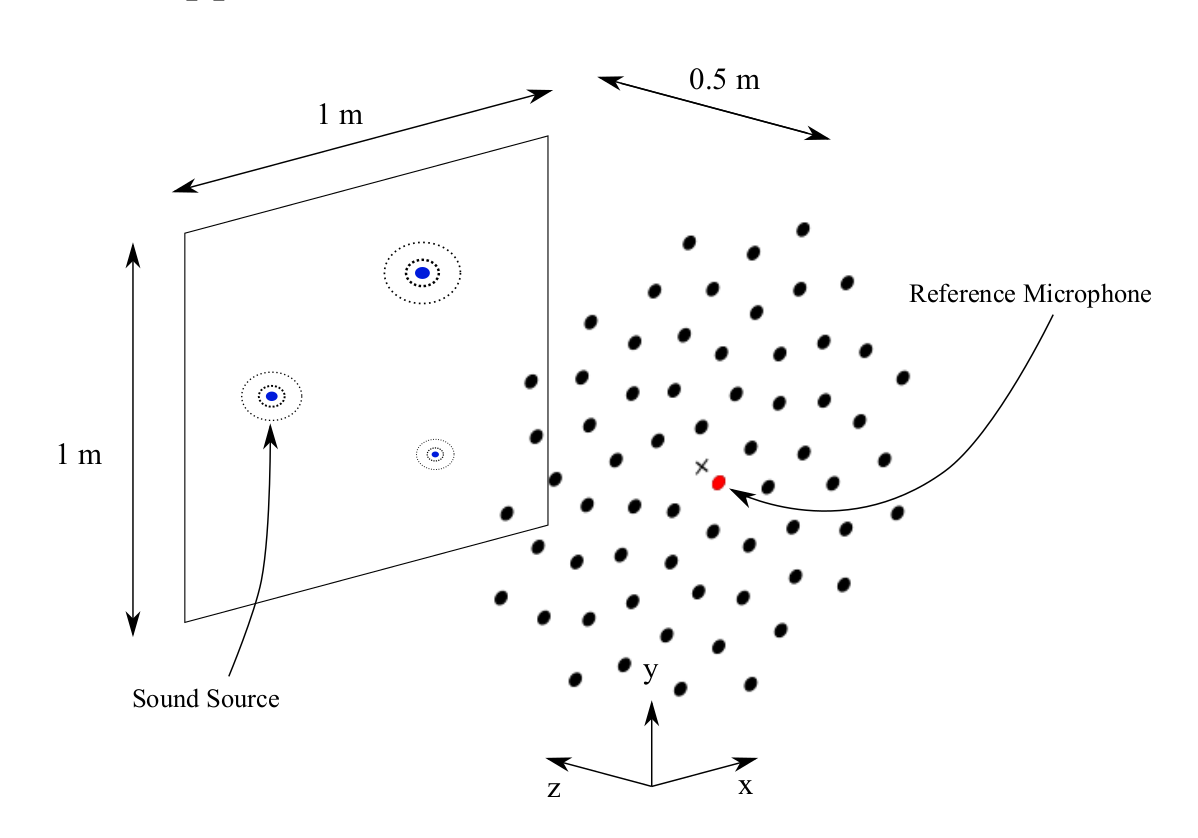
\includegraphics[width=0.65\textwidth]{../figs/full_measurement_setup.png}
    \caption{Example of the measurement setup used, with three audio sources}
    \label{fig:full_measurement_setup}
\end{figure} 

\begin{figure}
    \centering
    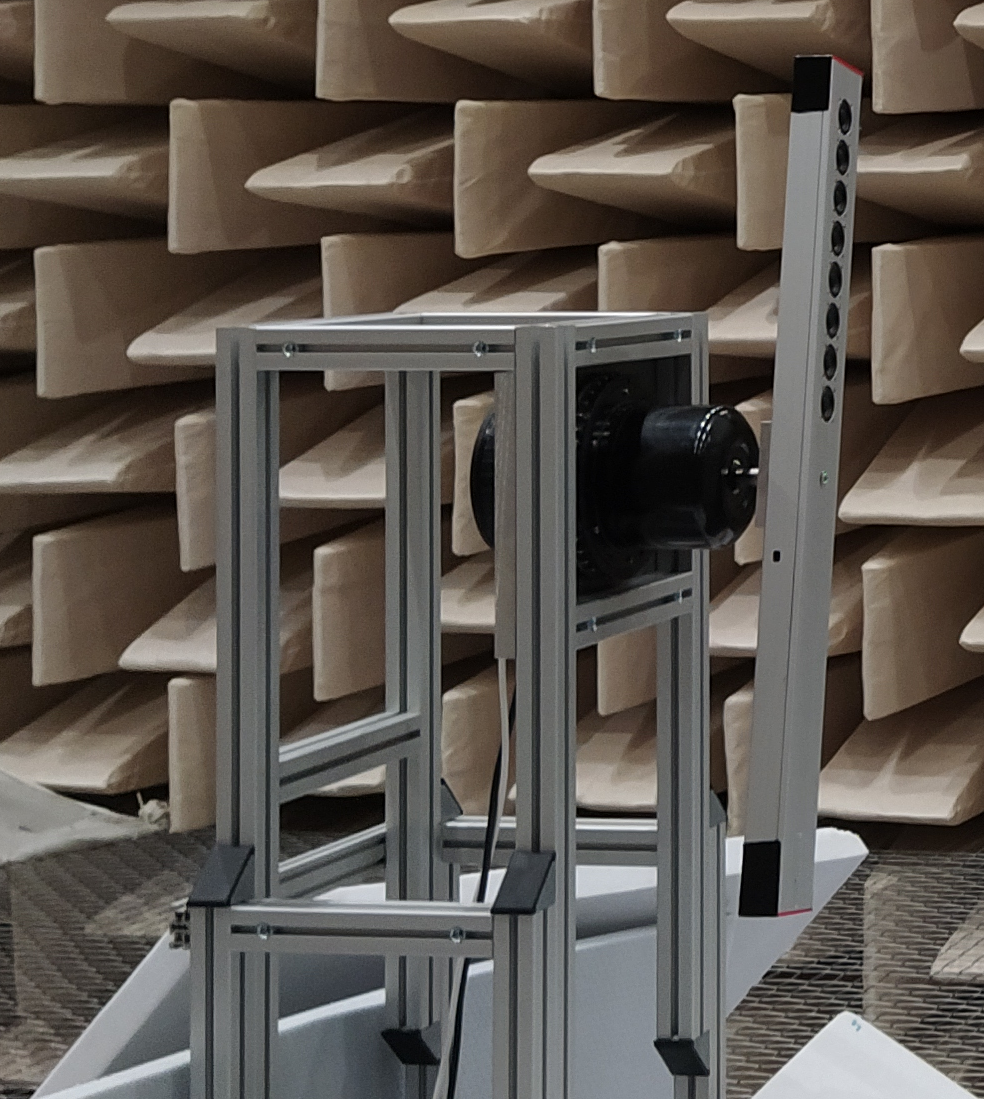
\includegraphics[width=0.65\textwidth]{../figs/source.png}
    \caption{Device used as audio source to create the measurement}
    \label{fig:source}
\end{figure}

\begin{figure}
    \centering
    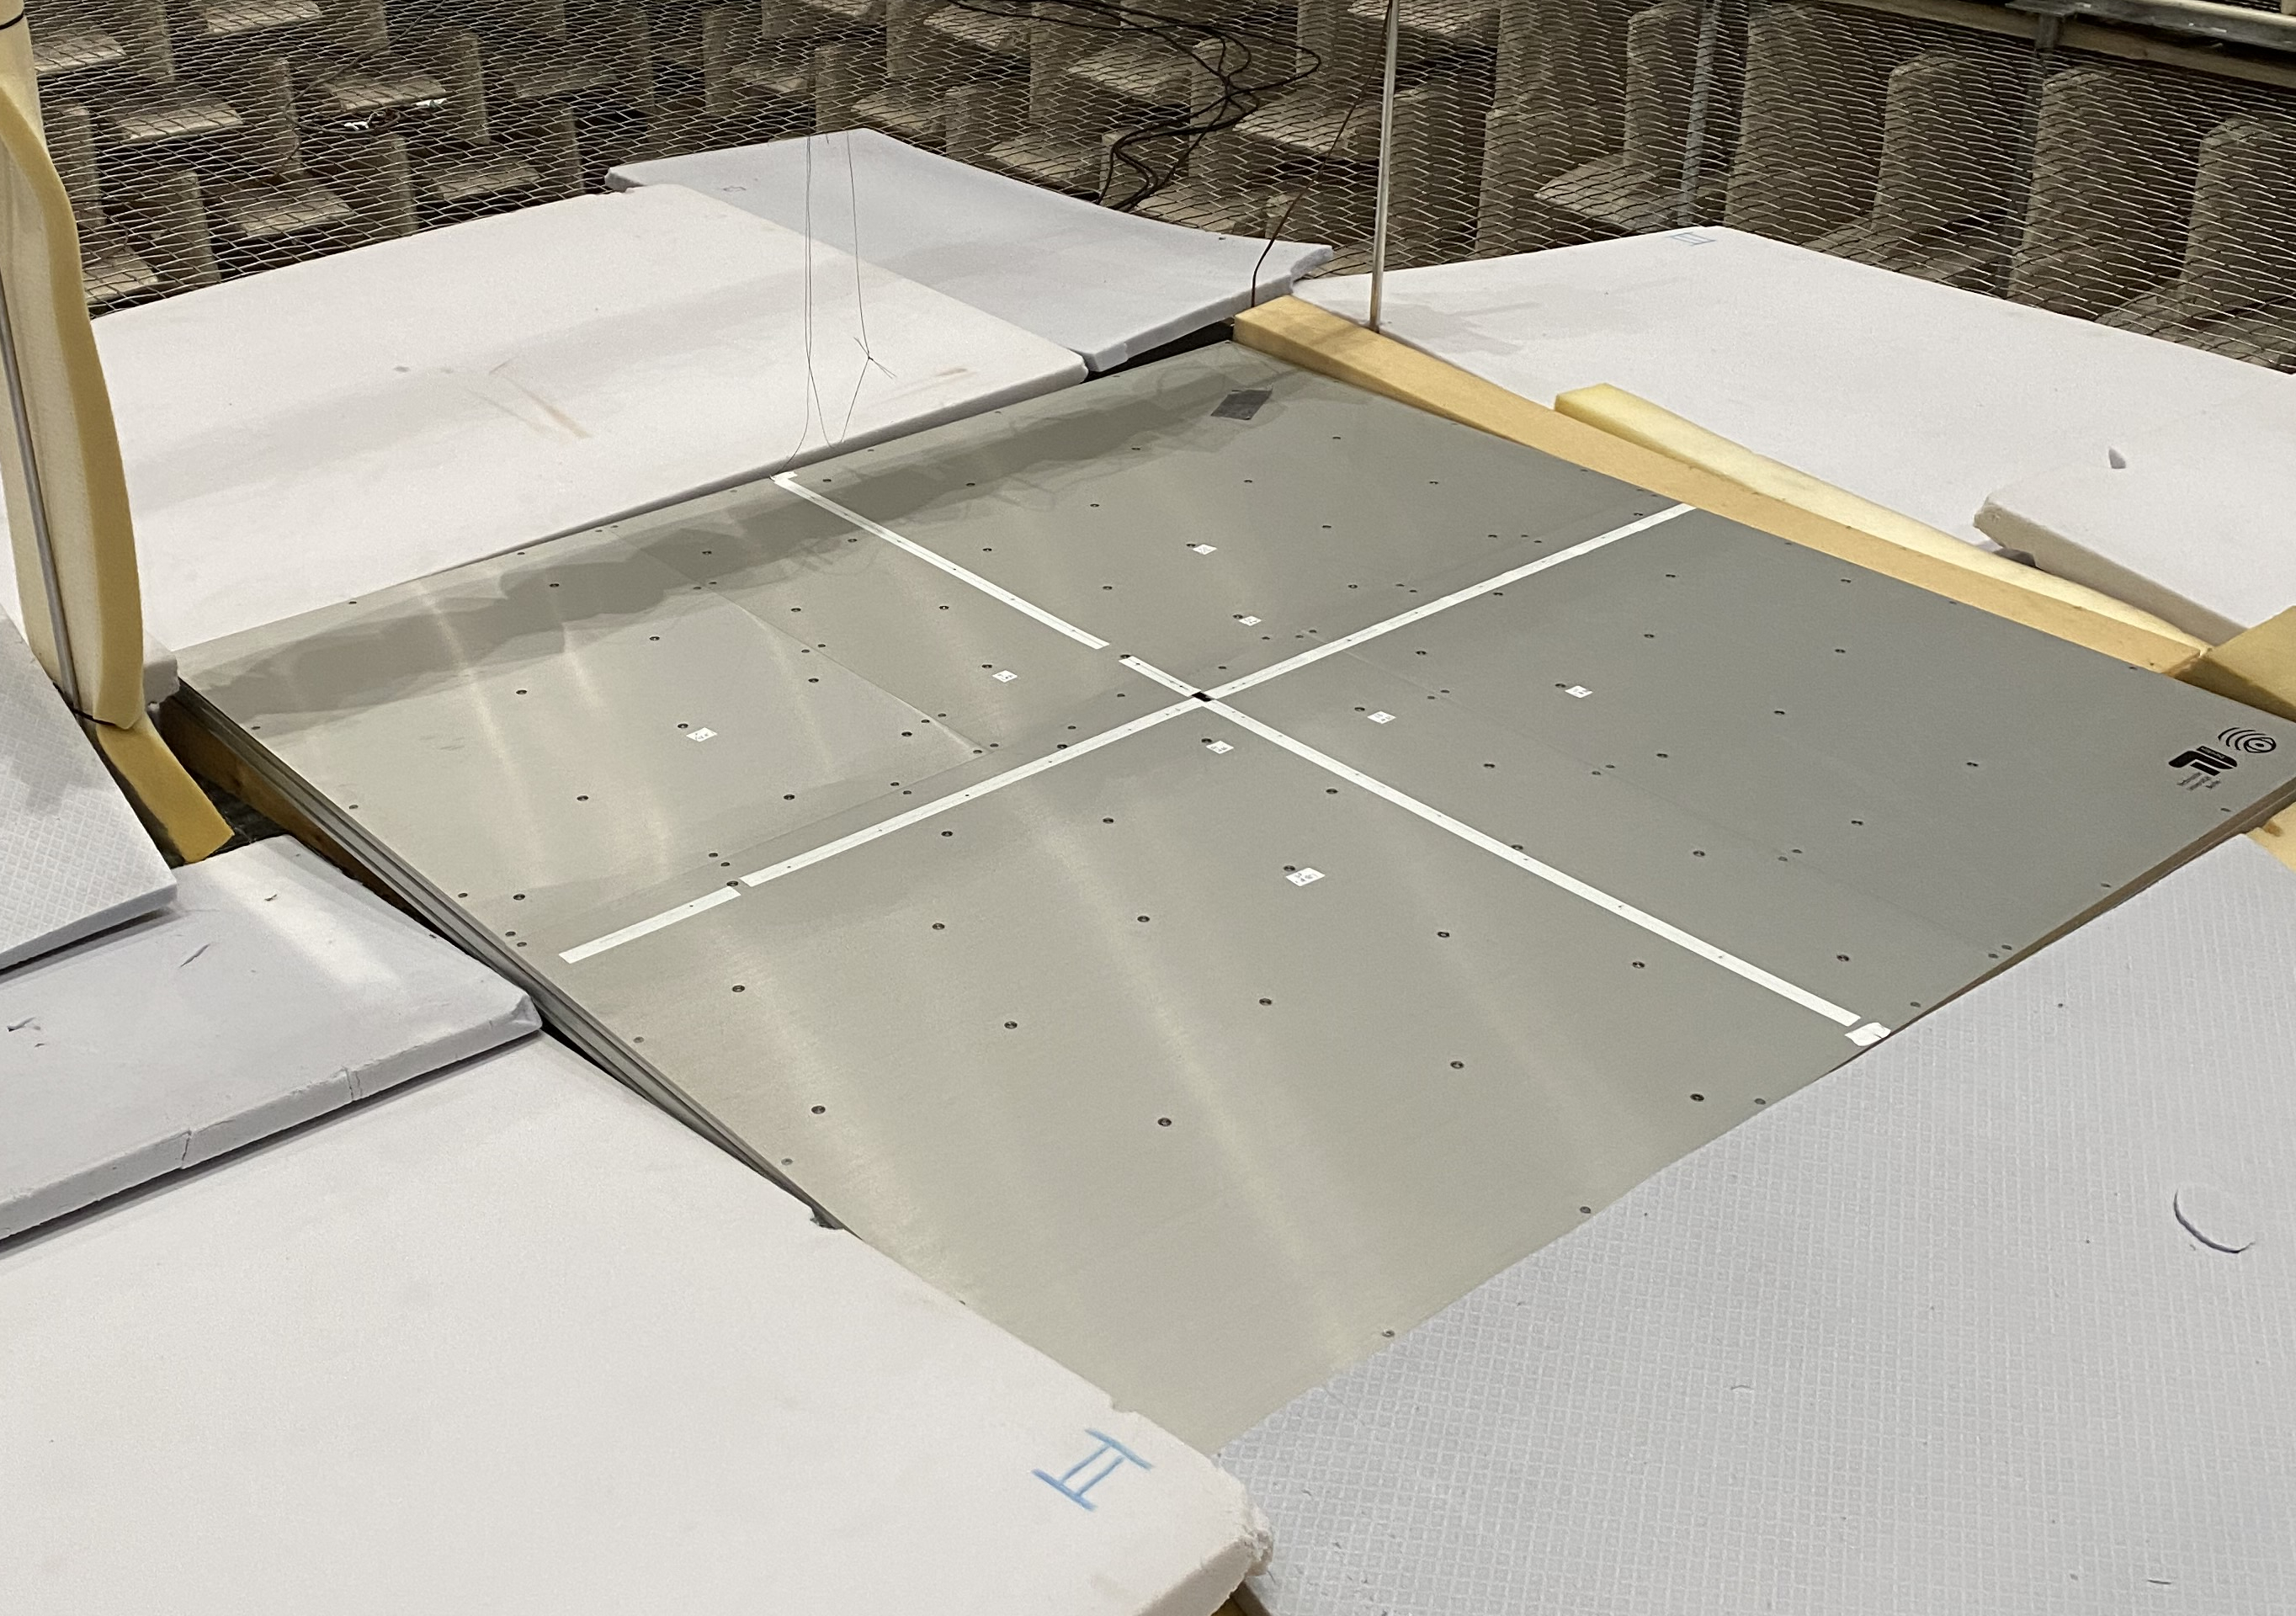
\includegraphics[width=0.65\textwidth]{../figs/microphone_array_cropped.jpg}
    \caption{Picture of the array of microphone used to create the real measurement}
    \label{fig:microphone_array}
\end{figure}

The measurements are sound pressure $\mathbf{p} \in \mathbb{C}^{64}$ at the 64 microphones of the array. Every recording is for a different position of the audio source. All measurements have a duration 10s and a sampling frequency of 51.2kHz.

From one measurement, we wanted to create many different approximation of the CSM $\hat{\mathbf{C}}$ to have enough data to fine tune our generative model. To do so, we took slices of $\frac{1}{50}$ of total measurement length (i.e. 0.2s). From this slice, $B$ snapshots needed to be created, for the approximation the CSM $\hat{\mathbf{C}}$ (see equation \ref{csm}). From \cite{gerstoft2012eigenvalues}, we know that the number of snapshots $B$ needed to be at least 4 times the number of receivers $M$ of the array (i.e. at least $4 \cdot 64 = 256$). For this purpose we used snapshots overlapping at 75\%. Indeed, \cite{gerstoft2012eigenvalues} argues that such a number of snapshots is required, for the eigenvalues of the approximated CSM $\hat{\mathbf{C}}$ to be sufficiently close to the eigenvalues of the real CSM $\mathbf{C}$ . Having snapshots overlapping at 75\% allowed us to have $B = 317 >  256$.

\textbf{Should something else be specified about the used microphones/loudspeaker?}: 



\subsubsection{Comparison between synthetic and measured data}

In Fig.\ref{fig:data_eigenvalue_spectrum}, we show a comparison of the normalized eigenvalues of a synthetic CSM compared with a measured CSM. In the synthetic eigenvalues, we observe first that all the eigenvalues except the first ones are close to zero. When observing the eigenspectrum of the measured data, a slowlier decay can be observed. We conclude that the measured and synthetic data are indeed not fully similar and hence that data synthetized in the above mentionned way cannot replaced measured data.

\begin{figure}
    \centering
    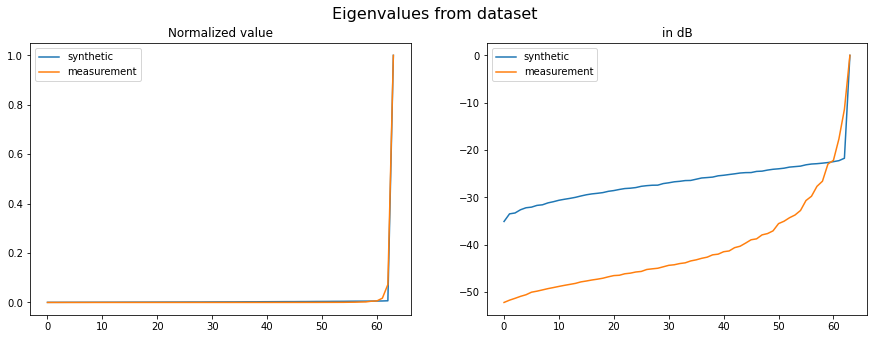
\includegraphics[width=\textwidth]{../figs/data_eigenvalue_spectrum.png}
    \caption{Comparison of the eigenvalues of CSMs approximated from synthetic data (blue) and from measured data (orange).}
    \label{fig:data_eigenvalue_spectrum}
\end{figure}

This can be explained by the fact that the synthetic CSM are closed to the perfection of a mathematical model and hence do not show presence of natural noise created by reverberation for instance.   


    


\subsection{Generation of Eigenvalues}

In order to generate the eigenvalue, a WGAN-GP was built. The implementation was adapted from \cite{nain2020wgangp}. Since the data to generate is the eigenvalues of CSMs of dimension $64 \times 64$, it is a vector $\mathbf{\lambda} \in \mathbb{R}^{64}$.

\subsubsection{Architecture}

As mentionned in the fundamentals the basic structure is two competing networks, a generator and a discriminator or critic. Both architectures of the generator and critic are illustrated respectively in tables Tab.\ref{tab:evals_generator_WGANGP_architecture} and Tab.\ref{tab:evals_critic_WGANGP_architecture}.

Unlike in the implementation of \cite{nain2020wgangp}, both inner networks (generator and critic) do not have a convolutional but a perceptron structure. Indeed, a convolutional structure is relevant when the data to generate is an image. Indeed, a convolutional layer is good at seeing patterns in image, by identifying topological structures in neighbouring pixels. We could have stacked pieces of our vector of eigenvalues $\mathbf{\lambda} = [\lambda_0, \dots, \lambda_{63}] \in \mathbb{R}^{64}$  into an image of dimension $8 \times 8$ but this would have resulted in an image where most neighbour pixel are not sharing any information about each other, hence making the convolutional operation irrelevant at detecting pattern, at least compared to images. 

Another changes that was made compared to the implementation of \cite{nain2020wgangp}, is that a ReLU actvation function was added as the last layer of the generator. Indeed before this change our generator would generate eigenvalues slightly smaller than zero. Moreover, we added 1e-100 ((\textbf{TODO: check actual value})) to every eigenvalue produced to ensure that they are positive.


\begin{table}[]
    \begin{tabular}{|l|l|l|}
        \hline
        \textbf{Layer (type)} & \textbf{Output Shape} & \textbf{Param \#} \\ \hline
        InputLayer            & (None, 128)           & 0                 \\ \hline
        Dense                 & (None, 256)           & 32768             \\ \hline
        LeakyReLU             & (None, 256)           & 0                 \\ \hline
        BatchNormalization    & (None, 256)           & 1024              \\ \hline
        Dense                 & (None, 512)           & 131584            \\ \hline
        LeakyReLU             & (None, 512)           & 0                 \\ \hline
        Dense                 & (None, 1024)          & 525312            \\ \hline
        LeakyReLU             & (None, 1024)          & 0                 \\ \hline
        Dense                 & (None, 64)            & 65600             \\ \hline
        \end{tabular}
    \caption{Architecture of the generator used in the WGAN-GP to generate eigenvalues. Total params: 756,288, Trainable params: 755,776, Non-trainable params: 512}
    \label{tab:evals_generator_WGANGP_architecture}
\end{table}

\begin{table}[]
    \begin{tabular}{|l|l|l|}
        \hline
        \textbf{Layer (type)} & \textbf{Output Shape} & \textbf{Param \#} \\ \hline
        InputLayer            & (None, 64)            & 0                 \\ \hline
        Dense                 & (None, 512)           & 33280             \\ \hline
        LeakyReLU             & (None, 512)           & 0                 \\ \hline
        Dense                 & (None, 256)           & 131328            \\ \hline
        LeakyReLU             & (None, 256)           & 0                 \\ \hline
        Dense                 & (None, 1)             & 257               \\ \hline
    \end{tabular}
    \caption{Architecture of the critic used in the WGAN-GP to generate eigenvalues. Total params: 164,865, Trainable params: 164,865, Non-trainable params: 0}
    \label{tab:evals_critic_WGANGP_architecture}
\end{table}


Finally, before being fed to the discriminator, real and generated eigenvalues are scaled such that $0 \leq \lambda_i \leq 1$ for $\lambda_i \in \mathbf{\lambda}$. Normalizing eigenvalues in this way is done to reduce the size of the sample space. This is illustrated in Fig.1\ref{fig:evals_wgangp_full_structure}.

\begin{figure}
    \centering
    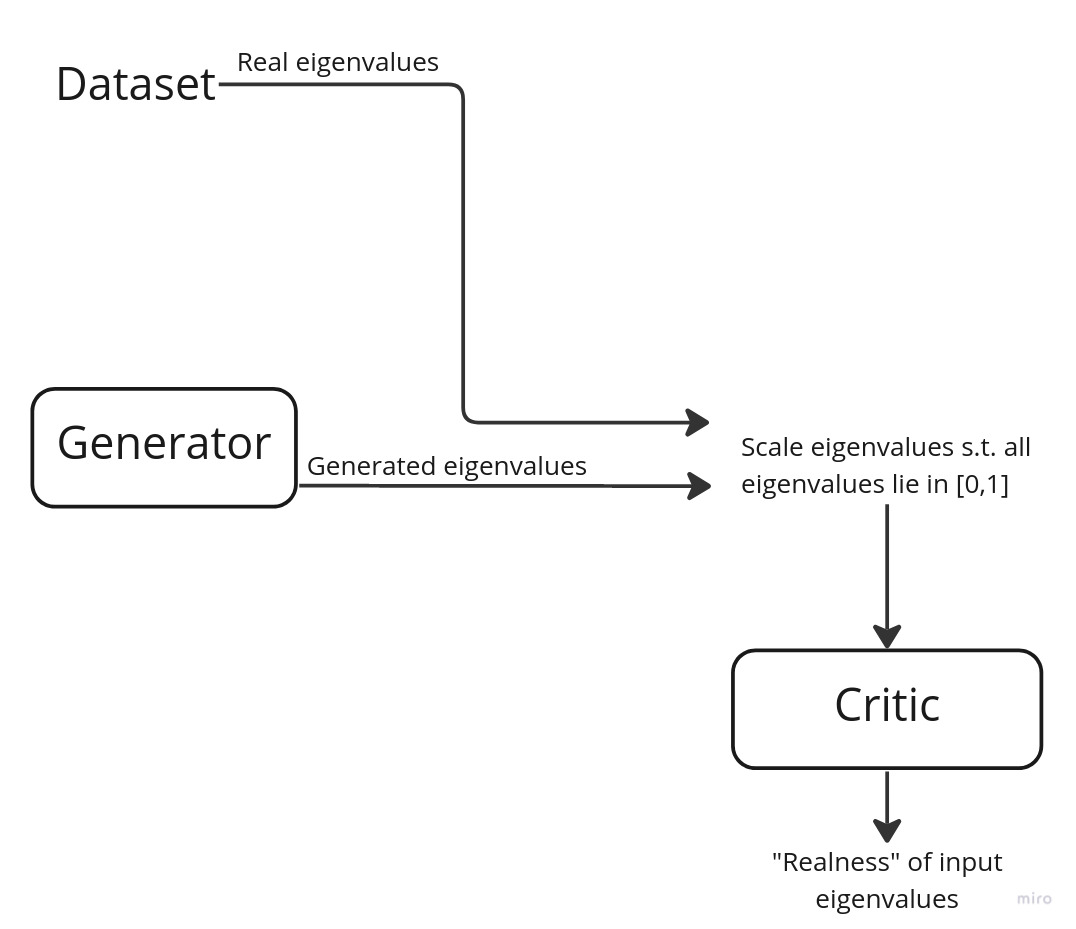
\includegraphics[width=0.65\textwidth]{../figs/evals_wgangp_full_structure.jpg}
    \caption{Full structure of the used implementation of the WGAN-GP to generate eigenvalues.}
    \label{fig:evals_wgangp_full_structure}
\end{figure}

\subsubsection{Results}

In Fig.\ref{fig:evals_wgangp_loss} and Fig.\ref{fig:evals_loss_after_finetuning}, we show the loss function when respectively training with the synthetic data and fine-tuing with measurement data. It can be observed that the model converged before the fine-tuning and that it did not have to change so much to adapt to generate measurement data, since the critic's loss function remain really close to zero. Moreover when comparing real  and generated eigenvalues sample in Fig.\ref{fig:eval_WGANGP_sample_before_fine_tuning} and Fig.\ref{fig:eval_WGANGP_sample_after_fine_tuning} (respectively before and after the fine-tuning), it can be observed that our WGAN-GP seem to produce sufficiently realisitic results, both for synthetic and measurement data.

\begin{figure}
    \centering
    \begin{minipage}{0.45\textwidth}
        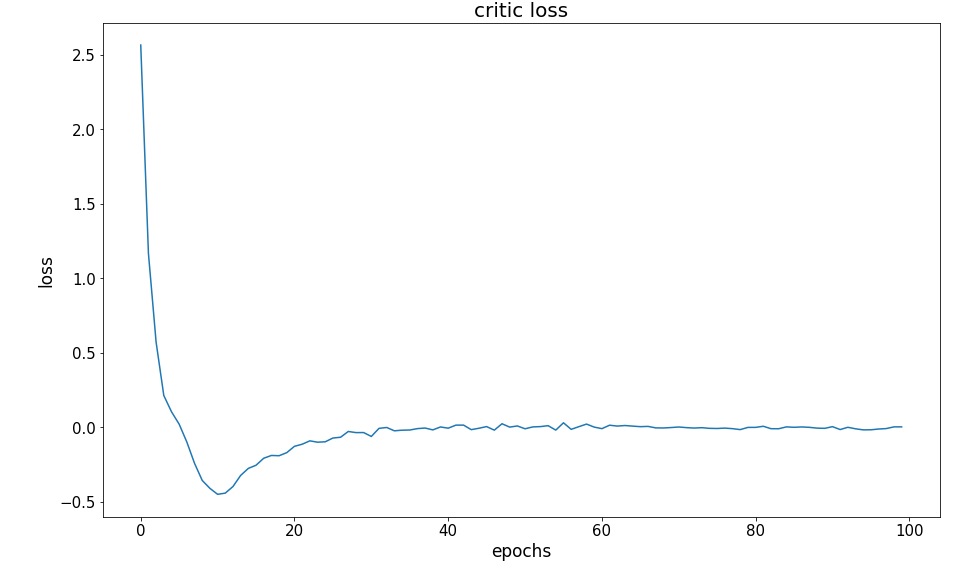
\includegraphics[width=0.9\textwidth]{../figs/evals_wgangp_loss.png}    
    \caption{The loss function of the critic while performing initial training of the WGAN-GP for eigenvalues generation (before fine-tuning).}
    \label{fig:evals_wgangp_loss}
    \end{minipage}\hfill
    \begin{minipage}{0.45\textwidth}
        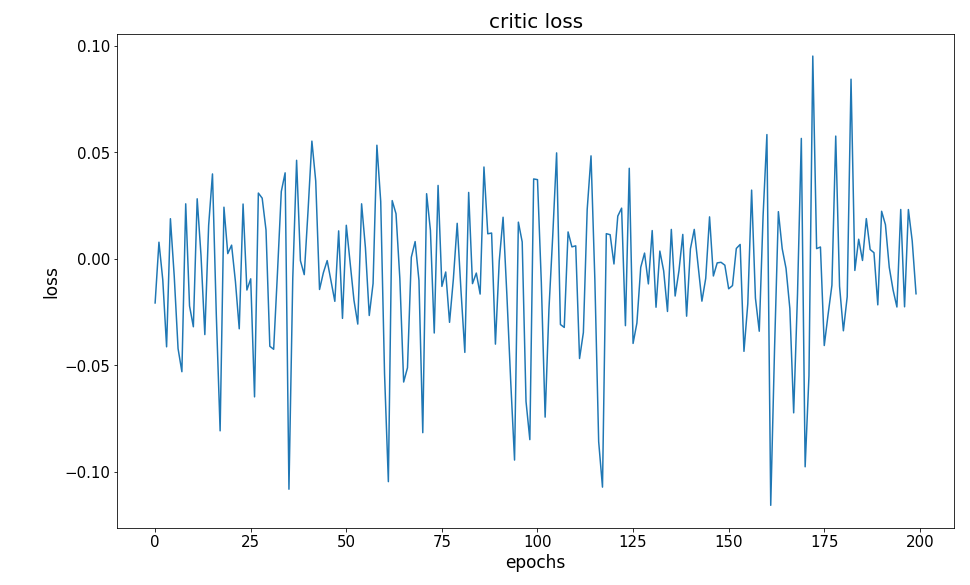
\includegraphics[width=0.9\textwidth]{../figs/evals_loss_after_finetuning.png}    
    \caption{The loss function of the critic while fine-tuning the WGAN-GP for eigenvalues generation.}
    \label{fig:evals_loss_after_finetuning}
    \end{minipage}
\end{figure}



\begin{figure}
    \centering
    \begin{minipage}{0.45\textwidth}
        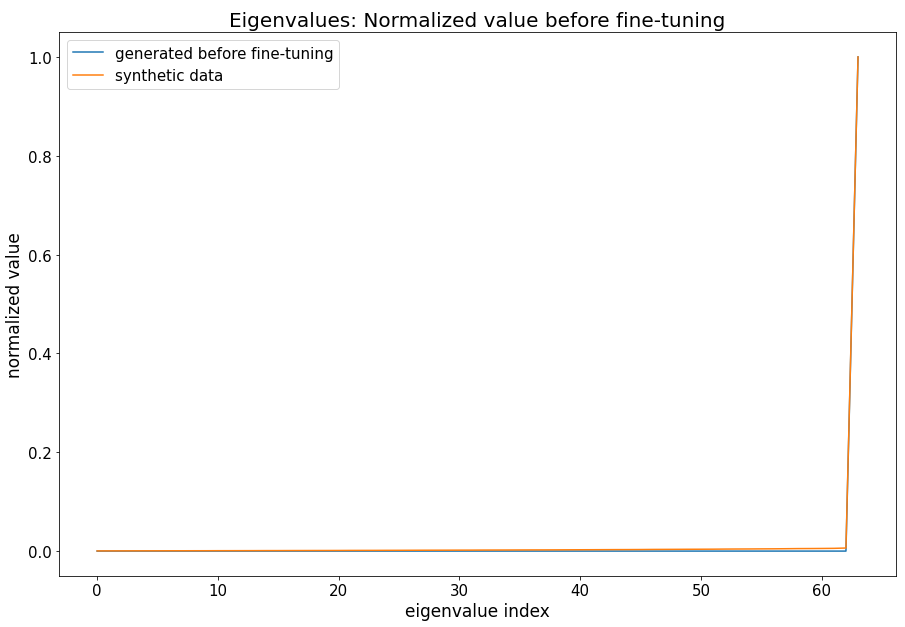
\includegraphics[width=1.2\textwidth]{../figs/eval_WGANGP_sample_before_fine_tuning.png}
        \caption{Comparision between real eigenvalues (orange) from the synthetic dataset with sample eigenvalues generated by our WGAN-GP (blue), when trained only with synthetic data (before fine-tuning)}
        \label{fig:eval_WGANGP_sample_before_fine_tuning}
    \end{minipage}\hfill
    \begin{minipage}{0.45\textwidth}
        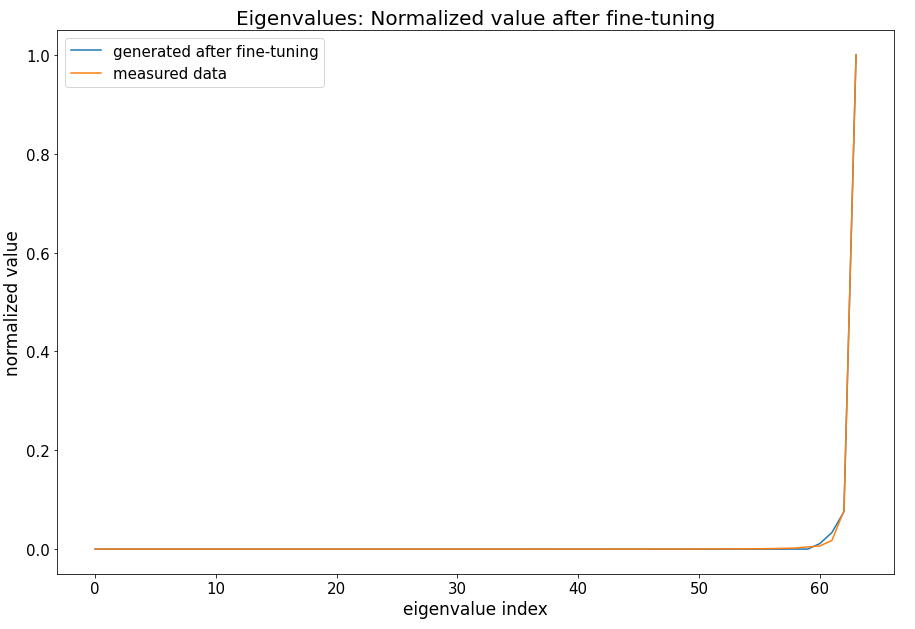
\includegraphics[width=1.2\textwidth]{../figs/eval_WGANGP_sample_after_fine_tuning.png}
        \caption{Comparision between real eigenvalues (orange) from the measurement dataset with sample eigenvalues generated by our WGAN-GP (blue), when trained further with measurement data (after fine-tuning)}
        \label{fig:eval_WGANGP_sample_after_fine_tuning}
    \end{minipage}
\end{figure}



But when we compare the level of the eigenvalue in Fig.\ref{fig:eval_WGANGP_sample_level}, it can easily be observed that the WGAN-GP struggles at generating eigenvalues around zero. More specifically, it can be easily observe that if we sort the eigenvalues such that $\lambda_0 \leq \lambda_0 \leq  \dots \leq \lambda_{63}$, then $\exists j>0$ s.t $\lambda_i = 10^{-10}$ $\forall i \leq j$. We remind that, by the way WGAN-GP has been implemented, $10^{-10}$ is the default minimum value. \textbf{TODO: write further}

\begin{figure}
    \centering
    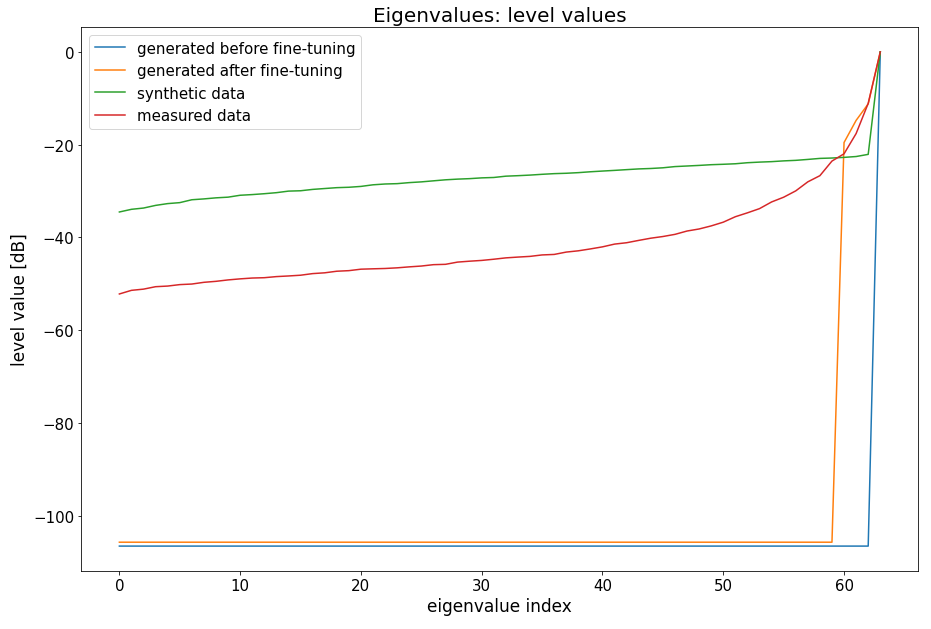
\includegraphics[width=0.9\textwidth]{../figs/eval_WGANGP_sample_level.png}    
    \caption{comparison level values of generated eigenvalues before fine-tuning (blue), generated eigenvalues after fine-tuning (orange) eigenvalues of synthetic CSM (green) and eigenvalues of CSM of measured data (red)}
    \label{fig:eval_WGANGP_sample_level}
\end{figure} 


\subsection{Generating eigenvalues from their level values}

As seen above, the WGAN-GP create convincing spectrum, until they are displayed as level. This led to idea of generating the spectrum from its levels values. We remind here how the level of the eigenvalues $[\lambda_0, \dots, \lambda_{63}] \in \Lambda$ are computed:

\begin{equation}
    L_{\lambda_i} = 10 \log_{10}(\frac{\lambda_i}{\lambda_{63}})
\end{equation}

where $\lambda_{63}$ is the biggest eigenvalue.

\subsubsection{Architecture}

The implementation was again inspired by \cite{nain2020wgangp}. More specifically, we adapted the networks created for generating directly the eigenvalues. Since all values $L_{\lambda_i}$ are non-positive, the generator has been built sucht that the two last steps are first a ReLU, followed by a multiplication by $-1$. This way we can ensure that our network only produces non-positive spectrum. This approach was also justified by the usage of Leaky ReLUs as activation throughout the generator. 

Because we were also using Leaky ReLUs in the critic, the first layer of its network is  also a multiplicative layer. Therefore, the critic is not trained to detect real from fake levels, but real from fake negative spectrum, which is equivalent.

The architecures used for the generator and the critic are shown respectively in Tab.\ref{tab:evals_dB_generator_WGANGP_architecture} and Tab.\ref{tab:evals_dB_critic_WGANGP_architecture}.

\begin{table}[]
    \begin{tabular}{|l|l|l|}
        \hline
        \textbf{Layer (type)} & \textbf{Output Shape} & \textbf{Param \#} \\ \hline
        InputLayer            & (None, 128)           & 0                 \\ \hline
        Dense                 & (None, 256)           & 32768             \\ \hline
        LeakyReLU             & (None, 256)           & 0                 \\ \hline
        BatchNormalization    & (None, 256)           & 1024              \\ \hline
        Dense                 & (None, 512)           & 131584            \\ \hline
        LeakyReLU             & (None, 512)           & 0                 \\ \hline
        Dense                 & (None, 1024)          & 525312            \\ \hline
        LeakyReLU             & (None, 1024)          & 0                 \\ \hline
        Dense                 & (None, 64)            & 65600             \\ \hline
        ReLU                  & (None, 64)            & 0                 \\ \hline
        Multiply              & (None, 64)            & 0                 \\ \hline
    \end{tabular}
    \caption{Architecture of the generator used in the WGAN-GP to generate eigenvalues from their level values. Total params: 756,288, Trainable params: 755,776, Non-trainable params: 512}
    \label{tab:evals_dB_generator_WGANGP_architecture}
\end{table}

\begin{table}[]
    \begin{tabular}{|l|l|l|}
        \hline
        \textbf{Layer (type)} & \textbf{Output Shape} & \textbf{Param \#} \\ \hline
        InputLayer            & (None, 64)            & 0                 \\ \hline
        Multiply              & (None, 64)            & 0                 \\ \hline
        Dense                 & (None, 512)           & 33280             \\ \hline
        LeakyReLU             & (None, 512)           & 0                 \\ \hline
        Dense                 & (None, 256)           & 131328            \\ \hline
        LeakyReLU             & (None, 256)           & 0                 \\ \hline
        Dense                 & None, 1               & 257               \\ \hline
    \end{tabular}
    \caption{Architecture of the critic used in the WGAN-GP to generate eigenvalues from their level values. Total params: 164,865, Trainable params: 164,865, Non-trainable params: 0}
    \label{tab:evals_dB_critic_WGANGP_architecture}
\end{table}

\subsubsection{Results}

When training this new WGANGP, the losses in Fig.\ref{fig:evals_dB_loss_before_finetuning} and Fig.\ref{fig:evals_dB_loss_after_finetuning} can be observed (respectively before and after fine-tuning). It can be seen that our model converged before fine-tuning, and it then had to adapt a bit during the fine-tuning but converged again.

\begin{figure}
    \centering
    \begin{minipage}{0.45\textwidth}
        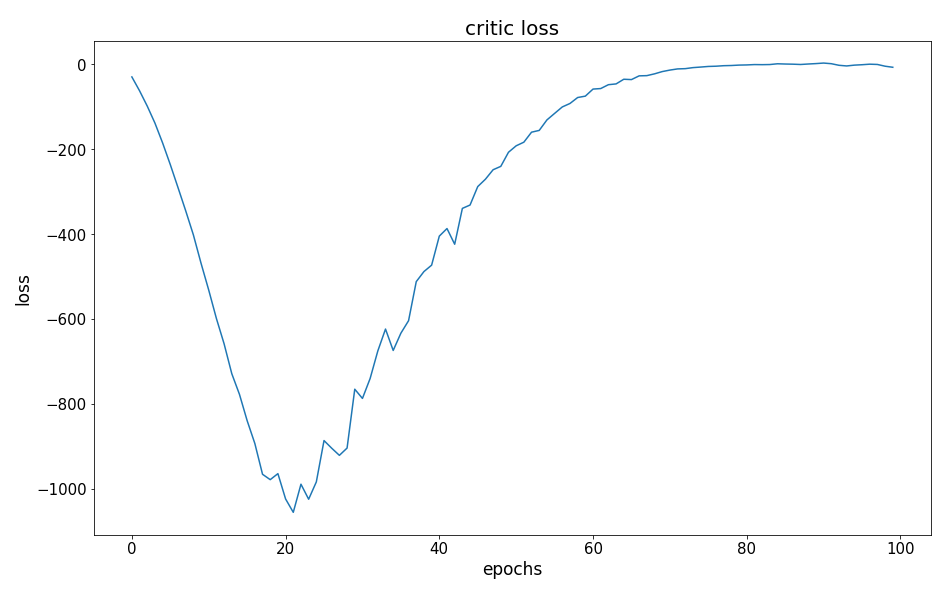
\includegraphics[width=0.9\textwidth]{../figs/evals_dB_loss_before_finetuning.png}    
    \caption{The loss function of the critic while performing initial training of the WGAN-GP for the levels of eigenvalues generation (before fine-tuning).}
    \label{fig:evals_dB_loss_before_finetuning}
    \end{minipage}\hfill
    \begin{minipage}{0.45\textwidth}
        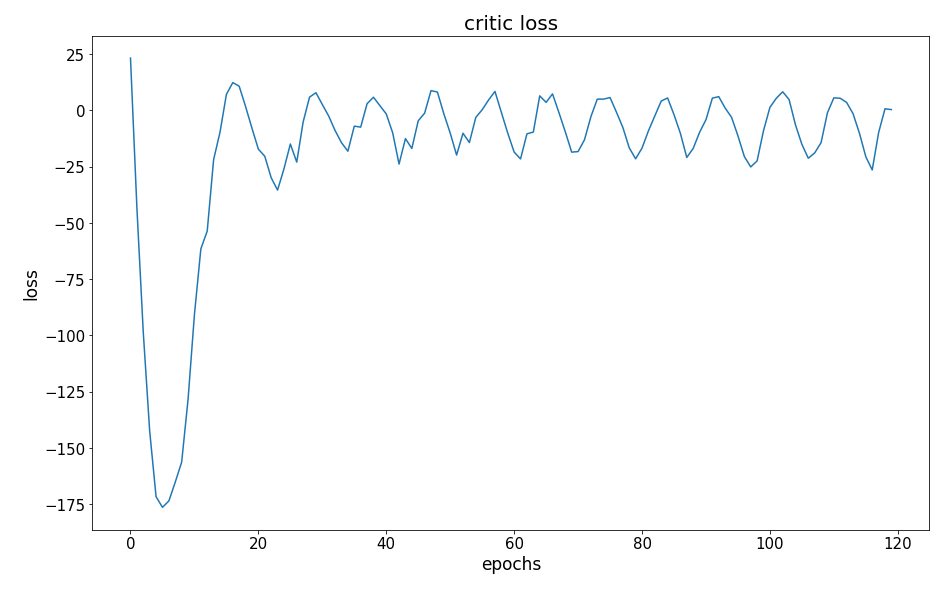
\includegraphics[width=0.9\textwidth]{../figs/evals_dB_loss_after_finetuning.png}    
    \caption{The loss function of the critic while fine-tuning the WGAN-GP for the levels of eigenvalues generation.}
    \label{fig:evals_dB_loss_after_finetuning}
    \end{minipage}
\end{figure}





In Fig.\ref{fig:evals_dB_sample_before_finetuning}, we show a comparison between real and generated levels of the eigenvalues of the CSM of synthetic data (before fine-tuning). We show in Fig.\ref{fig:evals_dB_sample_after_finetuning} the same comparison but after fine-tuning the WGAN-GP. It can observed that the obtained level samples look already more realistic than when the network is not trained with levels value of eigenvalues (see Fig.\ref{fig:eval_WGANGP_sample_level}).

\begin{figure}
    \centering
    \begin{minipage}{0.45\textwidth}
        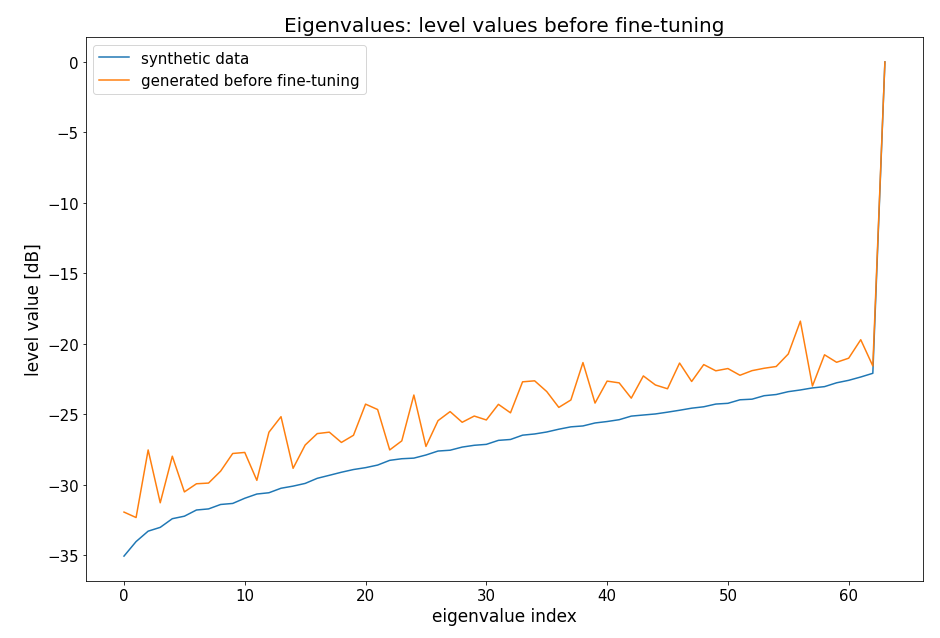
\includegraphics[width=1.2\textwidth]{../figs/evals_dB_sample_before_finetuning.png}
        \caption{Comparision between the levels of real eigenvalues (blue) from the synthetic dataset with sample levels eigenvalues generated by our WGAN-GP (orange), when trained only with synthetic data (before fine-tuning)}
        \label{fig:evals_dB_sample_before_finetuning}
    \end{minipage}\hfill
    \begin{minipage}{0.45\textwidth}
        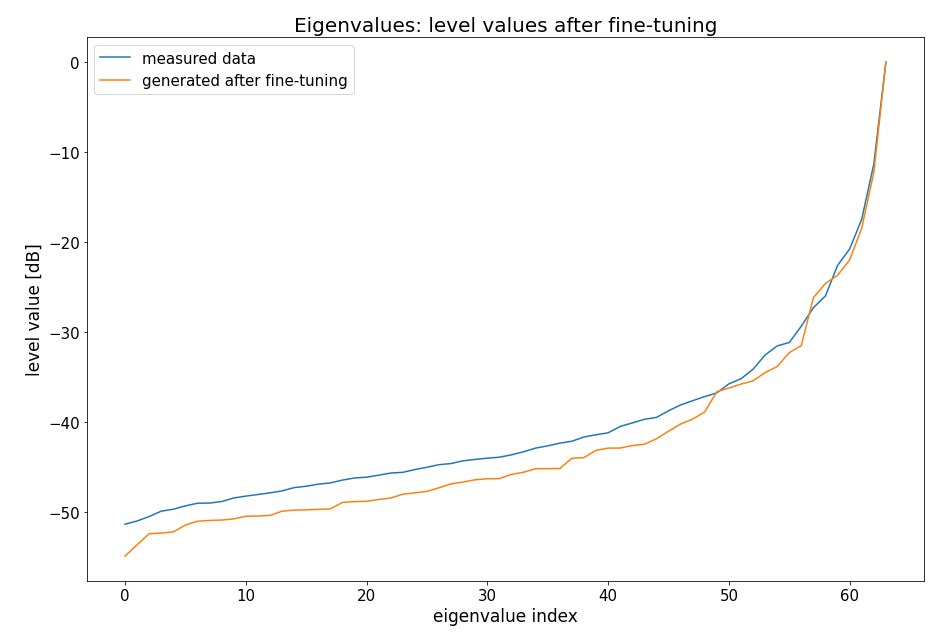
\includegraphics[width=1.2\textwidth]{../figs/evals_dB_sample_after_finetuning.png}
        \caption{Comparision between the levels real eigenvalues (blue) from the measurement dataset with sample levels of eigenvalues generated by our WGAN-GP (orange), when trained further with measurement data (after fine-tuning)}
        \label{fig:evals_dB_sample_after_finetuning}
    \end{minipage}
\end{figure}


Finally, we show in Fig.\ref{fig:evals_dB_not_level_sample_comparison} a comparison between the eigenvalues of eigenvalues of the CSM of measurement and the eigenvalues converted back from their level values. It can easily be observed that generating eigenvalues from their level values yields higher quality samples than when generating them directly.


\begin{figure}
    \centering
    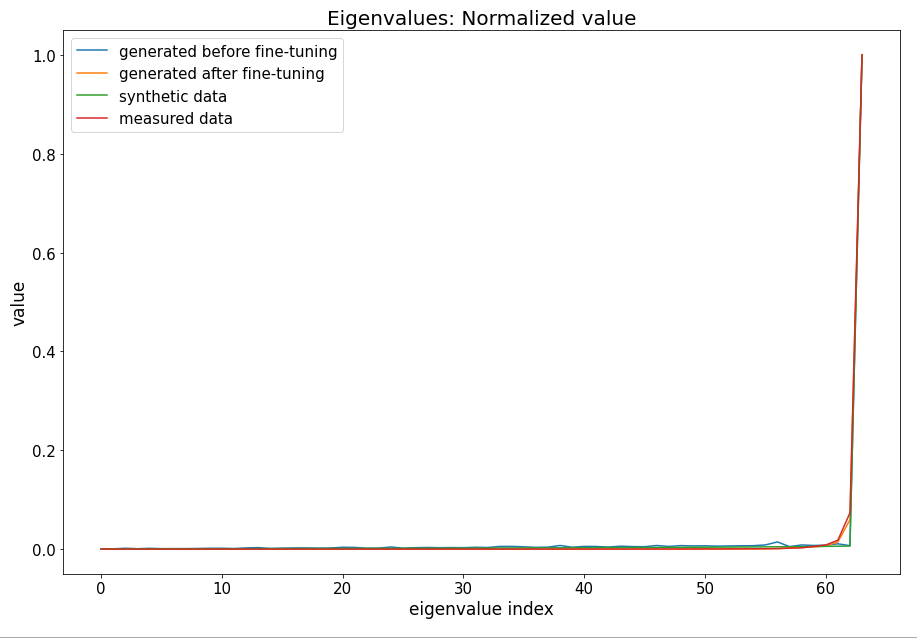
\includegraphics[width=0.9\textwidth]{../figs/evals_dB_not_level_sample_comparison.png}    
    \caption{comparison between generated eigenvalues before fine-tuning (blue), generated eigenvalues after fine-tuning (orange), eigenvalues of synthetic CSM (green) and eigenvalues of CSM of measured data (red). The eigenvalues are computed back from their level values.}
    \label{fig:evals_dB_not_level_sample_comparison}
\end{figure} 


\subsection{Generation of Eigenvectors}

The eigenvectors of the cross spectral were generated using two different GANs. The idea behind this not all vectors are sampled from the same distribution. Indeed there is only one main eigenvector (corresponding to a single DoA/source) and 63 "noise" vectors.  Each eigenvector belongs to a different source and all are incoherent. If there would to be  multiple coherent source, all the energy and their position merges into a single eigenmode. The main eigenvector is the one corresponding to the highest eigenvalues. Formally, the set of of all eigenvectors $\mathbf{V} \in \mathbb{C}^{64 \times 64}$ can be divided into two subsets $\mathbf{V}_{\text{main}} \in \mathbb{C}^{64 \times 1}$ and $\mathbf{V}_{\text{noise}} \in \mathbb{C}^{64 \times 63}$, with:

\begin{align}
    \mathbf{v}_{\text{main}} &\sim \mathbb{P}_{\text{main}} \\
    \mathbf{v}_{\text{noise}} &\sim \mathbb{P}_{\text{noise}}  
\end{align}

With $\mathbf{v}_{\text{main}} \in  \mathbf{V}_{\text{main}}$ and $\mathbf{v}_\text{noise} \in  \mathbf{V}_{\text{noise}}$ The above claim can be assessed visually. If we compare the values that the main vector and a noise eigenvector (randomly selecetd), we obtain the histogram respectively illustrated in Fig.\ref{fig:histogram_main_eigenvector} and Fig.\ref{fig:histogram_noise_eigenvector}. It can be seen that the values of the noise eigenvectors follows a gaussian distribution, whereas the values of the main eigenvector follows a more complex distribution.
 
\begin{figure}
    \centering
    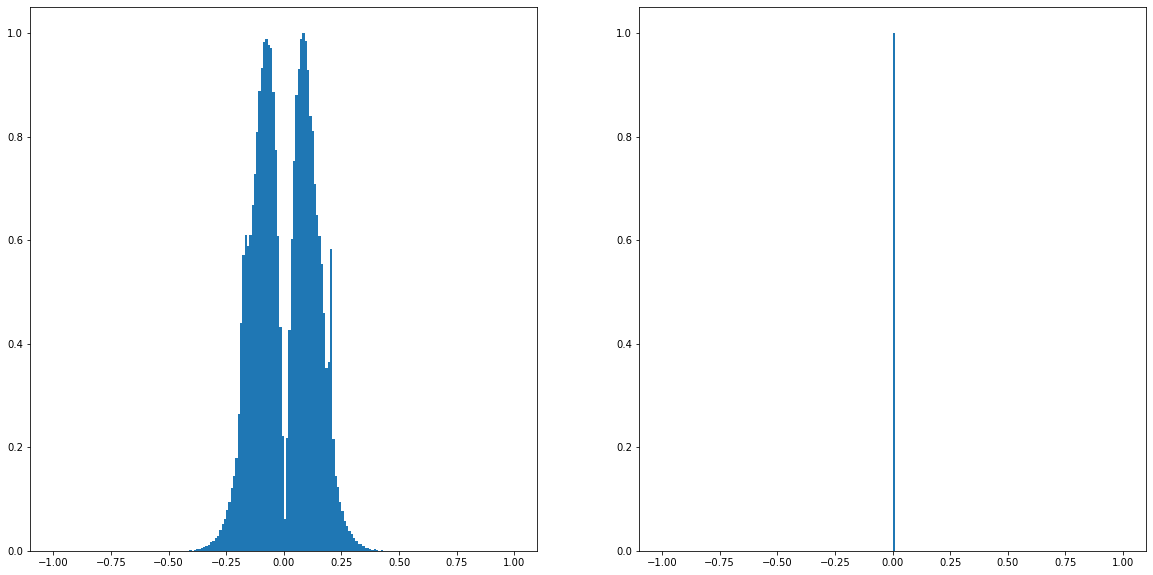
\includegraphics[width=0.65\textwidth]{../figs/histogram_main_eigenvector.png}
    \caption{histogram showing the value taken by the main eigenvector. The left side show the real part, whereas the right side shows the imaginary part.}
    \label{fig:histogram_main_eigenvector}
\end{figure}

\begin{figure}
    \centering
    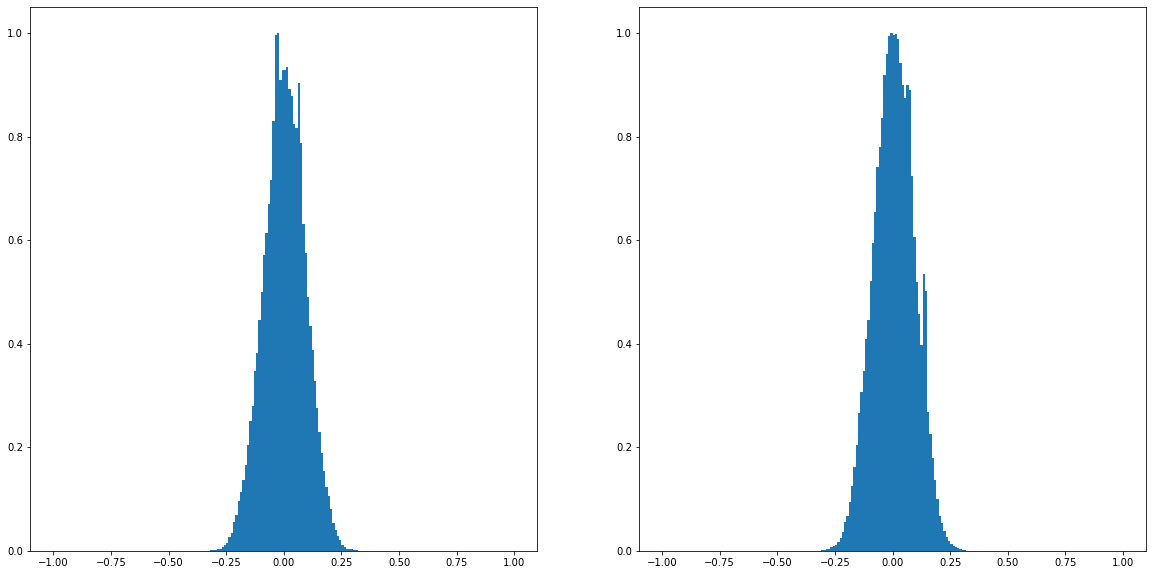
\includegraphics[width=0.65\textwidth]{../figs/histogram_noise_eigenvector.png}
    \caption{histogram shwoing the value taken by one of the noise eigenvector (selected at random). The left side show the real part, whereas the right side shows the imaginary part.}
    \label{fig:histogram_noise_eigenvector}
\end{figure}



% =====================================================================
% from mail: Yes, that makes sense. This  means that the information of multiple DOAs is included in a single eigenvector. Thus, as long as we are dealing with incoherent sources, your remark fully applies.
% =====================================================================


Similarly as for generating the eigenvalues, the eigenvectors were generated using a WGAN-GP whose implementation was adapted from \cite{nain2020wgangp}. Two different WGAN-GP were used to generate the two types of eigenvectors.

\subsection{WGAN-GP to generate the main eigenvector}

\subsubsection{Architecture}

First a WGAN-GP was created to generate the main eigenvector. Since it was simply a vector $\in \mathbb{C}^{64}$. It could be generated using a similar architecture as for the eigenvalues. The architectures both the generator and critic are illustrated respectively in the tables Tab.\ref{tab:main_evec_generator_WGANGP_architecture} and Tab.\ref{tab:main_evec_critic_WGANGP_architecture}.



\begin{table}[]
    \begin{tabular}{|l|l|l|}
        \hline
        \textbf{Layer (type)} & \textbf{Output Shape} & \textbf{Param \#} \\ \hline
        InputLayer            & (None, 128)           & 0                 \\ \hline
        Dense                 & (None, 256)           & 32768             \\ \hline
        LeakyReLU             & (None, 256)           & 0                 \\ \hline
        BatchNormalization    & (None, 256)           & 1024              \\ \hline
        Dense                 & (None, 512)           & 131584            \\ \hline
        LeakyReLU             & (None, 512)           & 0                 \\ \hline
        Dense                 & (None, 1024)          & 525312            \\ \hline
        LeakyReLU             & (None, 1024)          & 0                 \\ \hline
        Dense                 & (None, 128)           & 131200            \\ \hline
        Reshape               & (None, 1, 64, 2)      & 0                 \\ \hline
    \end{tabular}
    \caption{Architecture of the generator used in the WGAN-GP to generate the main eigenvector. Total params: 821,888, Trainable params: 821,376, Non-trainable params: 512}
    \label{tab:main_evec_generator_WGANGP_architecture}
\end{table}

\begin{table}[]
    \begin{tabular}{|l|l|l|}
        \hline
        \textbf{Layer (type)} & \textbf{Output Shape} & \textbf{Param \#} \\ \hline
        InputLayer            & (None, 1, 64, 2)      & 0                 \\ \hline
        Flatten               & (None, 128)           & 0                 \\ \hline
        Dense                 & (None, 512)           & 66048             \\ \hline
        LeakyReLU             & (None, 512)           & 0                 \\ \hline
        Dense                 & (None, 256)           & 131328            \\ \hline
        LeakyReLU             & (None, 256)           & 0                 \\ \hline
        Dense                 & (None, 1)             & 257               \\ \hline
    \end{tabular}
    \caption{Architecture of the critic used in the WGAN-GP to generate the main eigenvector. Total params: 197,633, Trainable params: 197,633, Non-trainable params: 0}
    \label{tab:main_evec_critic_WGANGP_architecture}
\end{table}



In order to reduce the sample space, both the real and generated main eigenvector are normalized before being fed to the discriminator. The full WGAN-GP structure is illutrates in Fig.\ref{fig:evecs_wgangp_full_structure}.


\begin{figure}
    \centering
    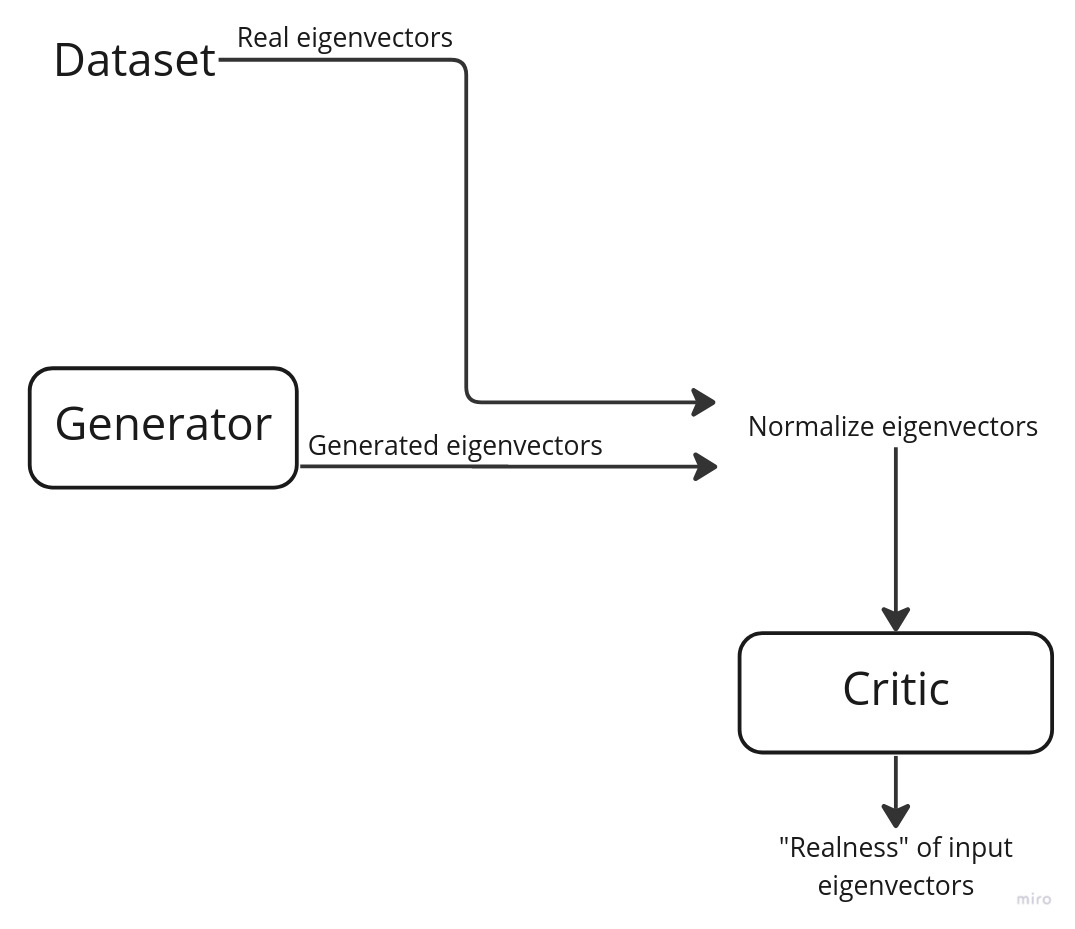
\includegraphics[width=0.65\textwidth]{../figs/evecs_wgangp_full_structure.jpg}
    \caption{Full structure of the used implementation of the WGAN-GP to generate eigenvectors.}
    \label{fig:evecs_wgangp_full_structure}
\end{figure}

\subsubsection{Results}

\textbf{TODO: to write when working}

\subsection{WGAN-GP to generate the noise eigenvectors \textbf{TODO: to see if it is only for noise eigenvectors, or for all evecs directly}}

\subsubsection{Architecture}

The approach used to generate the noise eigenvectors is similar as the main eigenvectors. The difference is that this time we wish to generate 63 vectors $\in mathbb{C}^64$. For this prupuse, we stack these 63 vector into a single vector $\in mathbb{C}^4032$. Due to the fact that we wish to generate a vector significantly larger, we add to increase the latent dimension from 128 to 4096 \textbf{TODO: this value need to be checked when the performance have been assessed}.

The architecture of both the generator and critic used are respectively shown in Tab.\ref{tab:noise_evecs_generator_WGANGP_architecture} and Tab.\ref{tab:noise_evecs_critic_WGANGP_architecture}. Similary as in the WGAN-GP for the main eigenvector, both real and generated eigenvector were normalized before being fed to the critic (see Fig.\ref{fig:evecs_wgangp_full_structure})


\begin{table}[]
    \begin{tabular}{|l|l|l|}
        \hline
        \textbf{Layer (Type)} & \textbf{Output Shape} & \textbf{Param \#} \\ \hline
        InputLayer            & (None, 128)           & 0                 \\ \hline
        Dense                 & (None, 256)           & 32768             \\ \hline
        BatchNormalization    & (None, 256)           & 1024              \\ \hline
        LeakyReLU             & (None, 256)           & 0                 \\ \hline
        Dense                 & (None, 1024)          & 262144            \\ \hline
        LeakyReLU             & (None, 1024)          & 0                 \\ \hline
        Dense                 & (None, 4096)          & 4194304           \\ \hline
        LeakyReLU             & (None, 4096)          & 0                 \\ \hline
        Dense                 & (None, 8064)          & 33030144          \\ \hline
        LeakyReLU             & (None, 8064)          & 0                 \\ \hline
        Reshape               & (None, 63, 64, 2)     & 0                 \\ \hline
    \end{tabular}
    \caption{Architecture of the generator used in the WGAN-GP to generate the noise eigenvectors. Total params: 37,520,384, Trainable params: 37,519,872, Non-trainable params: 512}
    \label{tab:noise_evecs_generator_WGANGP_architecture}
\end{table}

\begin{table}[]
    \begin{tabular}{|l|l|l|}
        \hline
        \textbf{Layer (Type)} & \textbf{Output Shape} & \textbf{Param \#} \\ \hline
        InputLayer            & (None, 63, 64, 2)     & 0                 \\ \hline
        Flatten               & (None, 8064)          & 0                 \\ \hline
        Dense                 & (None, 4096)          & 33034240          \\ \hline
        LeakyReLU             & (None, 4096)          & 0                 \\ \hline
        Dense                 & (None, 512)           & 2097664           \\ \hline
        LeakyReLU             & (None, 512)           & 0                 \\ \hline
        Dense                 & (None, 256)           & 131328            \\ \hline
        LeakyReLU             & (None, 256)           & 0                 \\ \hline
        Dense                 & (None, 1)             & 257               \\ \hline
        \end{tabular}
    \caption{Architecture of the critic used in the WGAN-GP to generate the noise eigenvectors. Total params: 35,263,489, Trainable params: 35,263,489, Non-trainable params: 0}
    \label{tab:noise_evecs_critic_WGANGP_architecture}
\end{table}

\subsubsection{Results}

\textbf{TODO: to write when working}

\subsection{Data Augmentation}

As seen before, we have some quite realistic looking generated eigenvalues. This led to the following idea for increasing the number of training samples (data augmentation). First, for a set of received CSM, decompose them in eigenvalues $\mathbf{\Lambda}$  and eigenvectors $\mathbf{V} = [\mathbf{v}_1^T, \dots, \mathbf{v}_M^T]$ with:

\begin{equation}
    \mathbf{\hat{C}} = \mathbf{V} \mathbf{\Lambda} \mathbf{V}^H
\end{equation}


The set of all eigenvalues can then be used to train a WGAN-GP. Using this network, we can generated eigenvalues $\hat{\mathbf{\Lambda}}$, which are realistic, up to an unknown scaling factor $c \in \mathbb{R}$.  


Then using the generated eigenvalues $\hat{\mathbf{\Lambda}}$ with real eigenvectors $\mathbf{V}$ we can have semi-generated CSM:

\begin{equation}
    \mathbf{\hat{C}}_\text{augm.}  = \mathbf{V} \hat{\mathbf{\Lambda}} \mathbf{V}^H
\end{equation}

which are realistic up to the scaling factor $c$. \textbf{TODO: show that the scaling factor $c$ does influence the beamforming}.

\subsubsection{Comparison between augmented data and real data.}


Fig.\ref{fig:beamforming_real_csm} and Fig.\ref{fig:beamforming_augmented_csm} show respectively the result of performing beamforming on a real CSM issued from the dataset and from a semi generated CSM. Both CSM have been recreated from the eigenvalue decomposition. It can be observed that both results are visually similar. A more careful obserbartion allows to notice that despite looking similar proportinaly, the overall values of in the beamforming map resulting from real data are slightly higher. This is due to the scaling of the eigenvalues taking place in the generative process. 

\begin{figure}
    \centering
    \begin{minipage}{0.45\textwidth}
        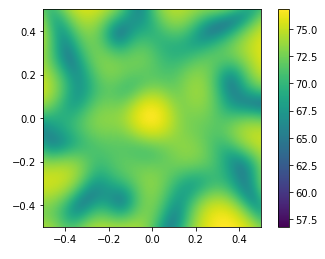
\includegraphics[width=1.2\textwidth]{../figs/beamforming_real_csm.png}
        \caption{Results of beamforming from a real CSM}
        \label{fig:beamforming_real_csm}
    \end{minipage}\hfill
    \begin{minipage}{0.45\textwidth}
        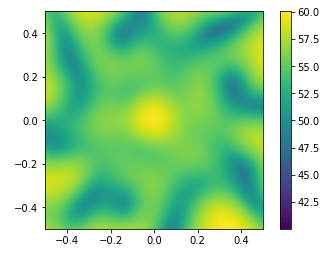
\includegraphics[width=1.2\textwidth]{../figs/beamforming_augmented_csm.png}
        \caption{Results of beamforming from a CSM issued from augmented data}
        \label{fig:beamforming_augmented_csm}
    \end{minipage}
\end{figure}

\subsection{Generation of Cross-Correlation Matrix}
% ========================================================================

\section{Conclusion}

\textbf{TODO: To write at the end}

\section{Future work}

\textbf{TODO}: here need to mention TransGAN, need to mention that the GAN could be made conditional 
    
% Bibliography
% Cite: version 1
%\printbibliography

 

% Cite: version 2
\bibliography{../mybib}
\bibliographystyle{plainnat}

\end{document}